% Options for packages loaded elsewhere
\PassOptionsToPackage{unicode}{hyperref}
\PassOptionsToPackage{hyphens}{url}
\PassOptionsToPackage{dvipsnames,svgnames,x11names}{xcolor}
%
\documentclass[
  authoryear,
  preprint,
  3p,
  onecolumn]{elsarticle}

\usepackage{amsmath,amssymb}
\usepackage{iftex}
\ifPDFTeX
  \usepackage[T1]{fontenc}
  \usepackage[utf8]{inputenc}
  \usepackage{textcomp} % provide euro and other symbols
\else % if luatex or xetex
  \usepackage{unicode-math}
  \defaultfontfeatures{Scale=MatchLowercase}
  \defaultfontfeatures[\rmfamily]{Ligatures=TeX,Scale=1}
\fi
\usepackage{lmodern}
\ifPDFTeX\else  
    % xetex/luatex font selection
\fi
% Use upquote if available, for straight quotes in verbatim environments
\IfFileExists{upquote.sty}{\usepackage{upquote}}{}
\IfFileExists{microtype.sty}{% use microtype if available
  \usepackage[]{microtype}
  \UseMicrotypeSet[protrusion]{basicmath} % disable protrusion for tt fonts
}{}
\makeatletter
\@ifundefined{KOMAClassName}{% if non-KOMA class
  \IfFileExists{parskip.sty}{%
    \usepackage{parskip}
  }{% else
    \setlength{\parindent}{0pt}
    \setlength{\parskip}{6pt plus 2pt minus 1pt}}
}{% if KOMA class
  \KOMAoptions{parskip=half}}
\makeatother
\usepackage{xcolor}
\setlength{\emergencystretch}{3em} % prevent overfull lines
\setcounter{secnumdepth}{5}
% Make \paragraph and \subparagraph free-standing
\ifx\paragraph\undefined\else
  \let\oldparagraph\paragraph
  \renewcommand{\paragraph}[1]{\oldparagraph{#1}\mbox{}}
\fi
\ifx\subparagraph\undefined\else
  \let\oldsubparagraph\subparagraph
  \renewcommand{\subparagraph}[1]{\oldsubparagraph{#1}\mbox{}}
\fi


\providecommand{\tightlist}{%
  \setlength{\itemsep}{0pt}\setlength{\parskip}{0pt}}\usepackage{longtable,booktabs,array}
\usepackage{calc} % for calculating minipage widths
% Correct order of tables after \paragraph or \subparagraph
\usepackage{etoolbox}
\makeatletter
\patchcmd\longtable{\par}{\if@noskipsec\mbox{}\fi\par}{}{}
\makeatother
% Allow footnotes in longtable head/foot
\IfFileExists{footnotehyper.sty}{\usepackage{footnotehyper}}{\usepackage{footnote}}
\makesavenoteenv{longtable}
\usepackage{graphicx}
\makeatletter
\def\maxwidth{\ifdim\Gin@nat@width>\linewidth\linewidth\else\Gin@nat@width\fi}
\def\maxheight{\ifdim\Gin@nat@height>\textheight\textheight\else\Gin@nat@height\fi}
\makeatother
% Scale images if necessary, so that they will not overflow the page
% margins by default, and it is still possible to overwrite the defaults
% using explicit options in \includegraphics[width, height, ...]{}
\setkeys{Gin}{width=\maxwidth,height=\maxheight,keepaspectratio}
% Set default figure placement to htbp
\makeatletter
\def\fps@figure{htbp}
\makeatother

\usepackage{lineno}\linenumbers \usepackage{multirow} \usepackage{lscape} \newcommand{\blandscape}{\begin{landscape}} \newcommand{\elandscape}{\end{landscape}}
\makeatletter
\makeatother
\makeatletter
\makeatother
\makeatletter
\@ifpackageloaded{caption}{}{\usepackage{caption}}
\AtBeginDocument{%
\ifdefined\contentsname
  \renewcommand*\contentsname{Table of contents}
\else
  \newcommand\contentsname{Table of contents}
\fi
\ifdefined\listfigurename
  \renewcommand*\listfigurename{List of Figures}
\else
  \newcommand\listfigurename{List of Figures}
\fi
\ifdefined\listtablename
  \renewcommand*\listtablename{List of Tables}
\else
  \newcommand\listtablename{List of Tables}
\fi
\ifdefined\figurename
  \renewcommand*\figurename{Figure}
\else
  \newcommand\figurename{Figure}
\fi
\ifdefined\tablename
  \renewcommand*\tablename{Table}
\else
  \newcommand\tablename{Table}
\fi
}
\@ifpackageloaded{float}{}{\usepackage{float}}
\floatstyle{ruled}
\@ifundefined{c@chapter}{\newfloat{codelisting}{h}{lop}}{\newfloat{codelisting}{h}{lop}[chapter]}
\floatname{codelisting}{Listing}
\newcommand*\listoflistings{\listof{codelisting}{List of Listings}}
\makeatother
\makeatletter
\@ifpackageloaded{caption}{}{\usepackage{caption}}
\@ifpackageloaded{subcaption}{}{\usepackage{subcaption}}
\makeatother
\makeatletter
\@ifpackageloaded{tcolorbox}{}{\usepackage[skins,breakable]{tcolorbox}}
\makeatother
\makeatletter
\@ifundefined{shadecolor}{\definecolor{shadecolor}{rgb}{.97, .97, .97}}
\makeatother
\makeatletter
\makeatother
\makeatletter
\makeatother
\journal{Journal Name}
\ifLuaTeX
  \usepackage{selnolig}  % disable illegal ligatures
\fi
\usepackage[]{natbib}
\bibliographystyle{elsarticle-harv}
\IfFileExists{bookmark.sty}{\usepackage{bookmark}}{\usepackage{hyperref}}
\IfFileExists{xurl.sty}{\usepackage{xurl}}{} % add URL line breaks if available
\urlstyle{same} % disable monospaced font for URLs
\hypersetup{
  pdftitle={Drought, vegetation productivity, and land cover change in Chile},
  pdfauthor={Francisco Zambrano; Anton Vrieling; Francisco Fernández; Francisco Meza; Alejandro Venegas-González; Iongel Duran-Llacer; Nicolas Raab; Dylan Craven},
  pdfkeywords={drought, land cover change, satellite},
  colorlinks=true,
  linkcolor={blue},
  filecolor={Maroon},
  citecolor={Blue},
  urlcolor={Blue},
  pdfcreator={LaTeX via pandoc}}

\setlength{\parindent}{6pt}
\begin{document}

\begin{frontmatter}
\title{Drought, vegetation productivity, and land cover change in Chile}
\author[1]{Francisco Zambrano%
\corref{cor1}%
\fnref{fn1}}
 \ead{francisco.zambrano@umayor.cl} 
\author[2]{Anton Vrieling%
%
}
 \ead{a.vrieling@utwente.nl} 
\author[3]{Francisco Fernández%
%
}
 \ead{a.vrieling@utwente.nl} 
\author[]{Francisco Meza%
%
}

\author[]{Alejandro Venegas-González%
%
}

\author[]{Iongel Duran-Llacer%
%
}

\author[]{Nicolas Raab%
%
}

\author[]{Dylan Craven%
%
}


\affiliation[1]{organization={Universidad Mayor, Hémera Centro de
Observación de la Tierra, Facultad de Ciencias, Escuela de Ingeniería en
Medio Ambiente y Sustentabilidad},city={Santiago,
Chile},postcode={7500994},postcodesep={}}
\affiliation[2]{organization={University of Twente, Faculty of
Geo-Information Science and Earth Observation (ITC)},city={Enschede, The
Netherlands},postcodesep={}}
\affiliation[3]{organization={Universidad San
Sebastian},,postcodesep={}}

\cortext[cor1]{Corresponding author}
\fntext[fn1]{This is the first author footnote.}







        
\begin{abstract}
Central Chile has been the focus of research studies due to the
persistent decrease in water supply, which is impacting the hydrological
system and vegetation development. This persistent period of water
scarcity has been defined as a megadrought. Our objective is to assess
the impact of drought on LULCC (land use land cover change) over
continental Chile using drought indices of water supply and demand, soil
moisture, and their impact on vegetation productivity. The monthly
ERA5-Land (ERA5L) variables for precipitation, temperature, and soil
moisture were used. From 2001 to 2022, we used the land cover MODIS
product MCD12Q1, and from 2000 to 2023, we used the NDVI (Normalized
Difference Vegetation Index) product MOD13A3 collection 6.1. As drought
indices, we compute the standardized anomaly of cumulative NDVI
(zcNDVI), the Standardized Precipitation Evapotranspiration Index
(SPEI), the Evaporative Demand Drought Index (EDDI), and the
Standardized Soil Moisture Index (SSI). These indices were calculated
for time scales of 1, 3, 6, 12, 24, and 36 months, except for zcNDVI,
which was for 6 months. We analyze the trend for LULCC, vegetation
productivity, and drought indices. Also, we analyzed the temporal
correlation of SPI, SPEI, EDDI, and SSI with zcNDVI to gain insights
into the impact of water supply and demand on vegetation productivity.
Our results showed that LULCC was highest in ``Centro,'' ``Sur,'' and
``Austral,'' with 36\%, 31\%, and 34\% of change in the surface type,
respectively. The EDDI shows that water demand has increased for all
zones, with a major increase in ``Norte Grande.'' The drought indices of
water supply and soil moisture evidence a decreasing trend, which
decreases at longer time scales, from ``Norte Grande'' to ``Sur.''
``Austral'' is the only zone that shows an increase in supply.
Vegetation productivity measures by zcNDVI present a negative trend in
``Norte Chico'' and ``Centro.'' On the other hand, forests seem to be
the most resistant to drought. The types that show to be most affected
by variation in climate conditions are shrublands, savannas, and
croplands. The drought indices that have the capability of explaining to
a major degree the variance in vegetation productivity are SSI-12,
followed by SPEI-24 and SPEI-12 in ``Norte Chico'' and ``Centro.'' The
results indicate that ``Norte Chico'' and ``Zona Central'' are the most
sensitive regions to water supply deficits lasting longer than a year.
Our results can help develop a robust vegetation productivity
forecasting model for land cover classes in Chile.
\end{abstract}





\begin{keyword}
    drought \sep land cover change \sep 
    satellite
\end{keyword}
\end{frontmatter}
    \captionsetup{justification=raggedright,singlelinecheck=false}

\ifdefined\Shaded\renewenvironment{Shaded}{\begin{tcolorbox}[sharp corners, breakable, boxrule=0pt, frame hidden, enhanced, interior hidden, borderline west={3pt}{0pt}{shadecolor}]}{\end{tcolorbox}}\fi

\hypertarget{introduction}{%
\section{Introduction}\label{introduction}}

Drought is often classified as meteorological when there is a decrease
in precipitation below the mean average of several years (more than 30
years), hydrological when these anomalies last for long periods (months
to years) and affect water systems, and agricultural when the deficit
impacts plant health anomalies and leads to decreased productivity
\citep{Wilhite1985}. However, it is important to note that drought is
also influenced by human activities, which were not considered in the
definitions. Thus, \citet{Loon2016} and \citet{AghaKouchak2021} have
given an updated definition of drought for the Anthropocene, suggesting
that it should be considered the feedback of humans' decisions and
activities that drives the anthropogenic drought. Simultaneously,
drought leads to heightened tree mortality and induces alterations in
land cover and land use, ultimately affecting ecosystems
\citep{Crausbay2017}. Even though many ecological studies have
misinterpreted how to characterize drought, for example, sometimes
considering ``dry'' conditions as ``drought'' \citep{Slette2019}. Then,
\citet{Crausbay2017} proposed the ecological drought definition as ``an
episodic deficit in water availability that drives ecosystems beyond
thresholds of vulnerability, impacts ecosystem services, and triggers
feedback in natural and/or human systems.'' In light of current global
warming, it is crucial to study the interaction between drought and
ecosystems in order to understand their feedback and impact on water
security. \citep{Bakker2012}

Human-induced greenhouse gas emissions have increased the frequency
and/or intensity of drought as a result of global warming, according to
the sixth assessment report (AR6) of the Intergovernmental Panel on
Climate Change (IPCC) \citep{IPCC2023}. The evidence supporting this
claim has been strengthened since AR5 \citep{IPCC2013}. Recent studies,
however, have produced contrasting findings, suggesting that drought has
not exhibited a significant trend over the past forty years.
\citep{Vicente-Serrano2022, Kogan2020}. \citet{Vicente-Serrano2022}
analyzed the meteorological drought trend on a global scale, finding
that only in a few regions has there been an increase in the severity of
drought. Moreover, they attribute the increase in droughts over the past
forty years solely to an increase in atmospheric evaporative demand
(AED), which in turn enhances vegetation water demand, with important
implications for agricultural and ecological droughts. Also, they state
that ``the increase in hydrological droughts has been primarily observed
in regions with high water demand and land cover change''. Similarly,
\citet{Kogan2020} analyzed the drought trend using vegetation health
methods, finding that for the globe, hemispheres, and main
grain-producing countries, drought has not expanded or intensified for
the last 38 years. Further, the \citet{IPCC2021} suggests that there is
a high degree of confidence that rising temperatures will increase the
extent, frequency, and severity of droughts. Also, AR6 \citep{IPCC2023}
predicts that many regions of the world will experience more severe
agricultural and ecological droughts even if global warming stabilizes
at 1.5°--2°C. To better evaluate the impact of drought trends on
ecosystems, assessments are needed that relate meteorological and soil
moisture variables to their effects on vegetation.

From 1960 to 2019, land use change has impacted around one-third of the
Earth's surface, which is four times more than previously thought
\citep{Winkler2021}. Multiple studies aim to analyze and forecast
changes in land cover globally \citep{Winkler2021, Song2018} and
regionally \citep{Chamling2020, Homer2020, Yang2021}. Some others seek
to analyze the impact of land cover change on climate conditions such as
temperature and precipitation \citep{Luyssaert2014, Pitman2012}. There
is less research on the interaction between drought and land cover
change \citep{Chen2022, Akinyemi2021, Peng2017}. \citet{Peng2017}
conducted a worldwide investigation utilizing net primary production to
examine the spatial and temporal variations in vegetation productivity
at global level. The study aimed to assess the influence of drought by
comparing the twelve-month Standardized Precipitation Evapotranspiration
Index (SPEI) and land cover change. According to their findings, drought
is responsible for 37\% of the decline in vegetation productivity, while
water availability accounts for 55\% of the variation. \citet{Chen2022}
studied the trend of vegetation greenness and productivity and its
relation to meteorological drought (SPEI of twelve months in December)
and soil moisture at the global level. The results showed lower
correlations (\textless0.2) for both variables. \citet{Akinyemi2021}
evaluates drought trends and land cover change using vegetation indices
in Botwsana in a semi-arid climate. These studies mostly looked at how
changes in land cover and vegetation productivity are related to a
single drought index (SPEI) over a single time period of 12 months. SPEI
takes into account the combined effect of precipitation and AED as a
water balance, but it does not allow us to know the contribution of each
variable on its own. Some things worth investigating in terms of land
cover change and vegetation productivity are: i) How do they respond to
short- to long-term meteorological droughts? ii) How do they behave in
humid and arid climatic zones regarding drought? And iii) What is the
role of soil moisture? Likewise, there is a lack of understanding of how
the alteration in water supply and demand is affecting land cover
transformations.

Chile's diverse climatic and ecosystem types
(\citet{Beck2023};\citet{Luebert2022}) make it an ideal natural
laboratory for studying climate and ecosystems. Additionally, the
country has experienced severe drought conditions that have had
significant effects on vegetation and water storage. Central Chile faced
a persistent precipitation deficit between 2010 and 2022, defined as a
megadrought \citep{Garreaud2017}, which has impacted the Chilean
ecosystem. This megadrought was defined by the Standardized
Precipitation Index (SPI) of twelve months in December having values
below one standard deviation. Some studies have addressed how this
drought affects single ecosystems in terms of forest development
\citep{Miranda2020, Venegas2018}, forest fire occurrence
\citep{UrrutiaJalabert2018}, and crop productivity
\citep{Zambrano2023, Zambrano2018, Zambrano2016}. We found one study
regarding land cover and drought in Chile. The study by
\citet{Fuentes2021} evaluates water scarcity and land cover change in
Chile between 29° and 39° of south latitude. \citet{Fuentes2021} used
the SPEI of one month for evaluating drought, which led to misleading
results. For example, they did not find a temporal trend in the SPEI but
found a decreasing trend in water availability and an increase trend on
AED, which in turn should have been capable of being captured with
longer time scales of the SPEI. The term ``megadrought'' in Chile is
used to describe a prolonged water shortage that lasts for several
years, resulting in a permanent deficit that impacts the hydrological
system \citep{Boisier2018}. Hence, it is imperative to assess temporal
scales that take into account the cumnulative effect within some years.
There is little knowledge about the relationship between drought and
ecosystem in Chile; thus, it is important to understand in more detail
how meteorological and soil moisture droughts influence ecosystem
dynamics to inform adaptation options.

A detailed spatiotemporal assessment of the interaction of drought for
short- to long-term and land cover change requires information on
vegetation as well as weather variables such as precipitation,
temperature, and soil moisture. Weather networks in Chile present some
disadvantages, such as spatio-temporal gaps, a short history, and
irregular quality, which make them difficult to represent the whole
extent of the country spatially. In order to do this, we use reanalysis
data from ERA5-Land \citep{MunozSabater2021} to create drought indices
that consider AED, precipitation, and soil moisture over a range of time
periods, from the short to the long term. Also, we use vegetation
spectral information and annual land cover change from the
Moderate-Resolution Imaging Spectroradiometer (MODIS). We expect to gain
insight regarding the temporal evolution of water demand, water supply,
and soil moisture, as well as the interaction with land cover change and
vegetation productivity. Here, we analyze the multi-dimensional impacts
of drought across ecosystems in continental Chile. More specifically, we
aim to assess: i) temporal changes in land-use cover and the direction
and magnitude of their relationships with drought indices for water
demand and supply, soil moisture, and vegetation productivity; ii)
short- to long-term temporal trends in multi-scalar drought indices; and
iii) the relationship between vegetation productivity and drought
indices for water demand and supply and soil moisture across Chilean
ecosystems.

\hypertarget{study-area}{%
\section{Study area}\label{study-area}}

Continental Chile has a diverse climate conditions with strong gradients
from north to south and east to west \citep{Aceituno2021}
(Figure~\ref{fig-studyArea} a), which determines its great ecosystem
diversity (\citet{Luebert2022}) (Figure~\ref{fig-studyArea} c). The
Andes Mountains are a main factor in climate latitudinal variation
\citep{Garreaud2009}. In order to characterize the climate and ecosystem
of Chile, we utilize the Köppen-Geiger classification system developed
by \citet{Beck2023} and the land cover data derived from the MODIS
product for the period of 2001--2022, based on the International
Geosphere-Biosphere Programme (IGBP) classification scheme proposed by
\citet{Friedl2019}. ``Norte Grande'' and ``Norte Chico'' predominate in
an arid desert climate with hot (Bwh) and cold (Bwk) temperatures. At
the south of ``Norte Chico,'' the climate changes to an arid steppe with
cold temperatures (Bsk). In these two northern regions, the land is
mostly bare, with a minor surface of vegetation types such as shrubland
and grassland. In the zones ``Centro'' and the north half of ``Sur,''
the main climate is Mediterranean, with warm to hot summers (Csa and
Csb). Land cover in ``Centro'' comprises a significant amount of
shrubland and savanna (50\%), grassland (16\%), forest (8\%), and
croplands (5\%). An oceanic climate (Cfb) predominates in the south of
``Sur'' and the north of ``Austral.'' Those zones are high in forest and
grassland. The southern part of the country has a tundra climate, and in
``Austral'', it is a cold semi-arid area with an extended surface of
grassland, forest, and, to a lesser extent, savanna.

\begin{figure*}[!ht]

{\centering 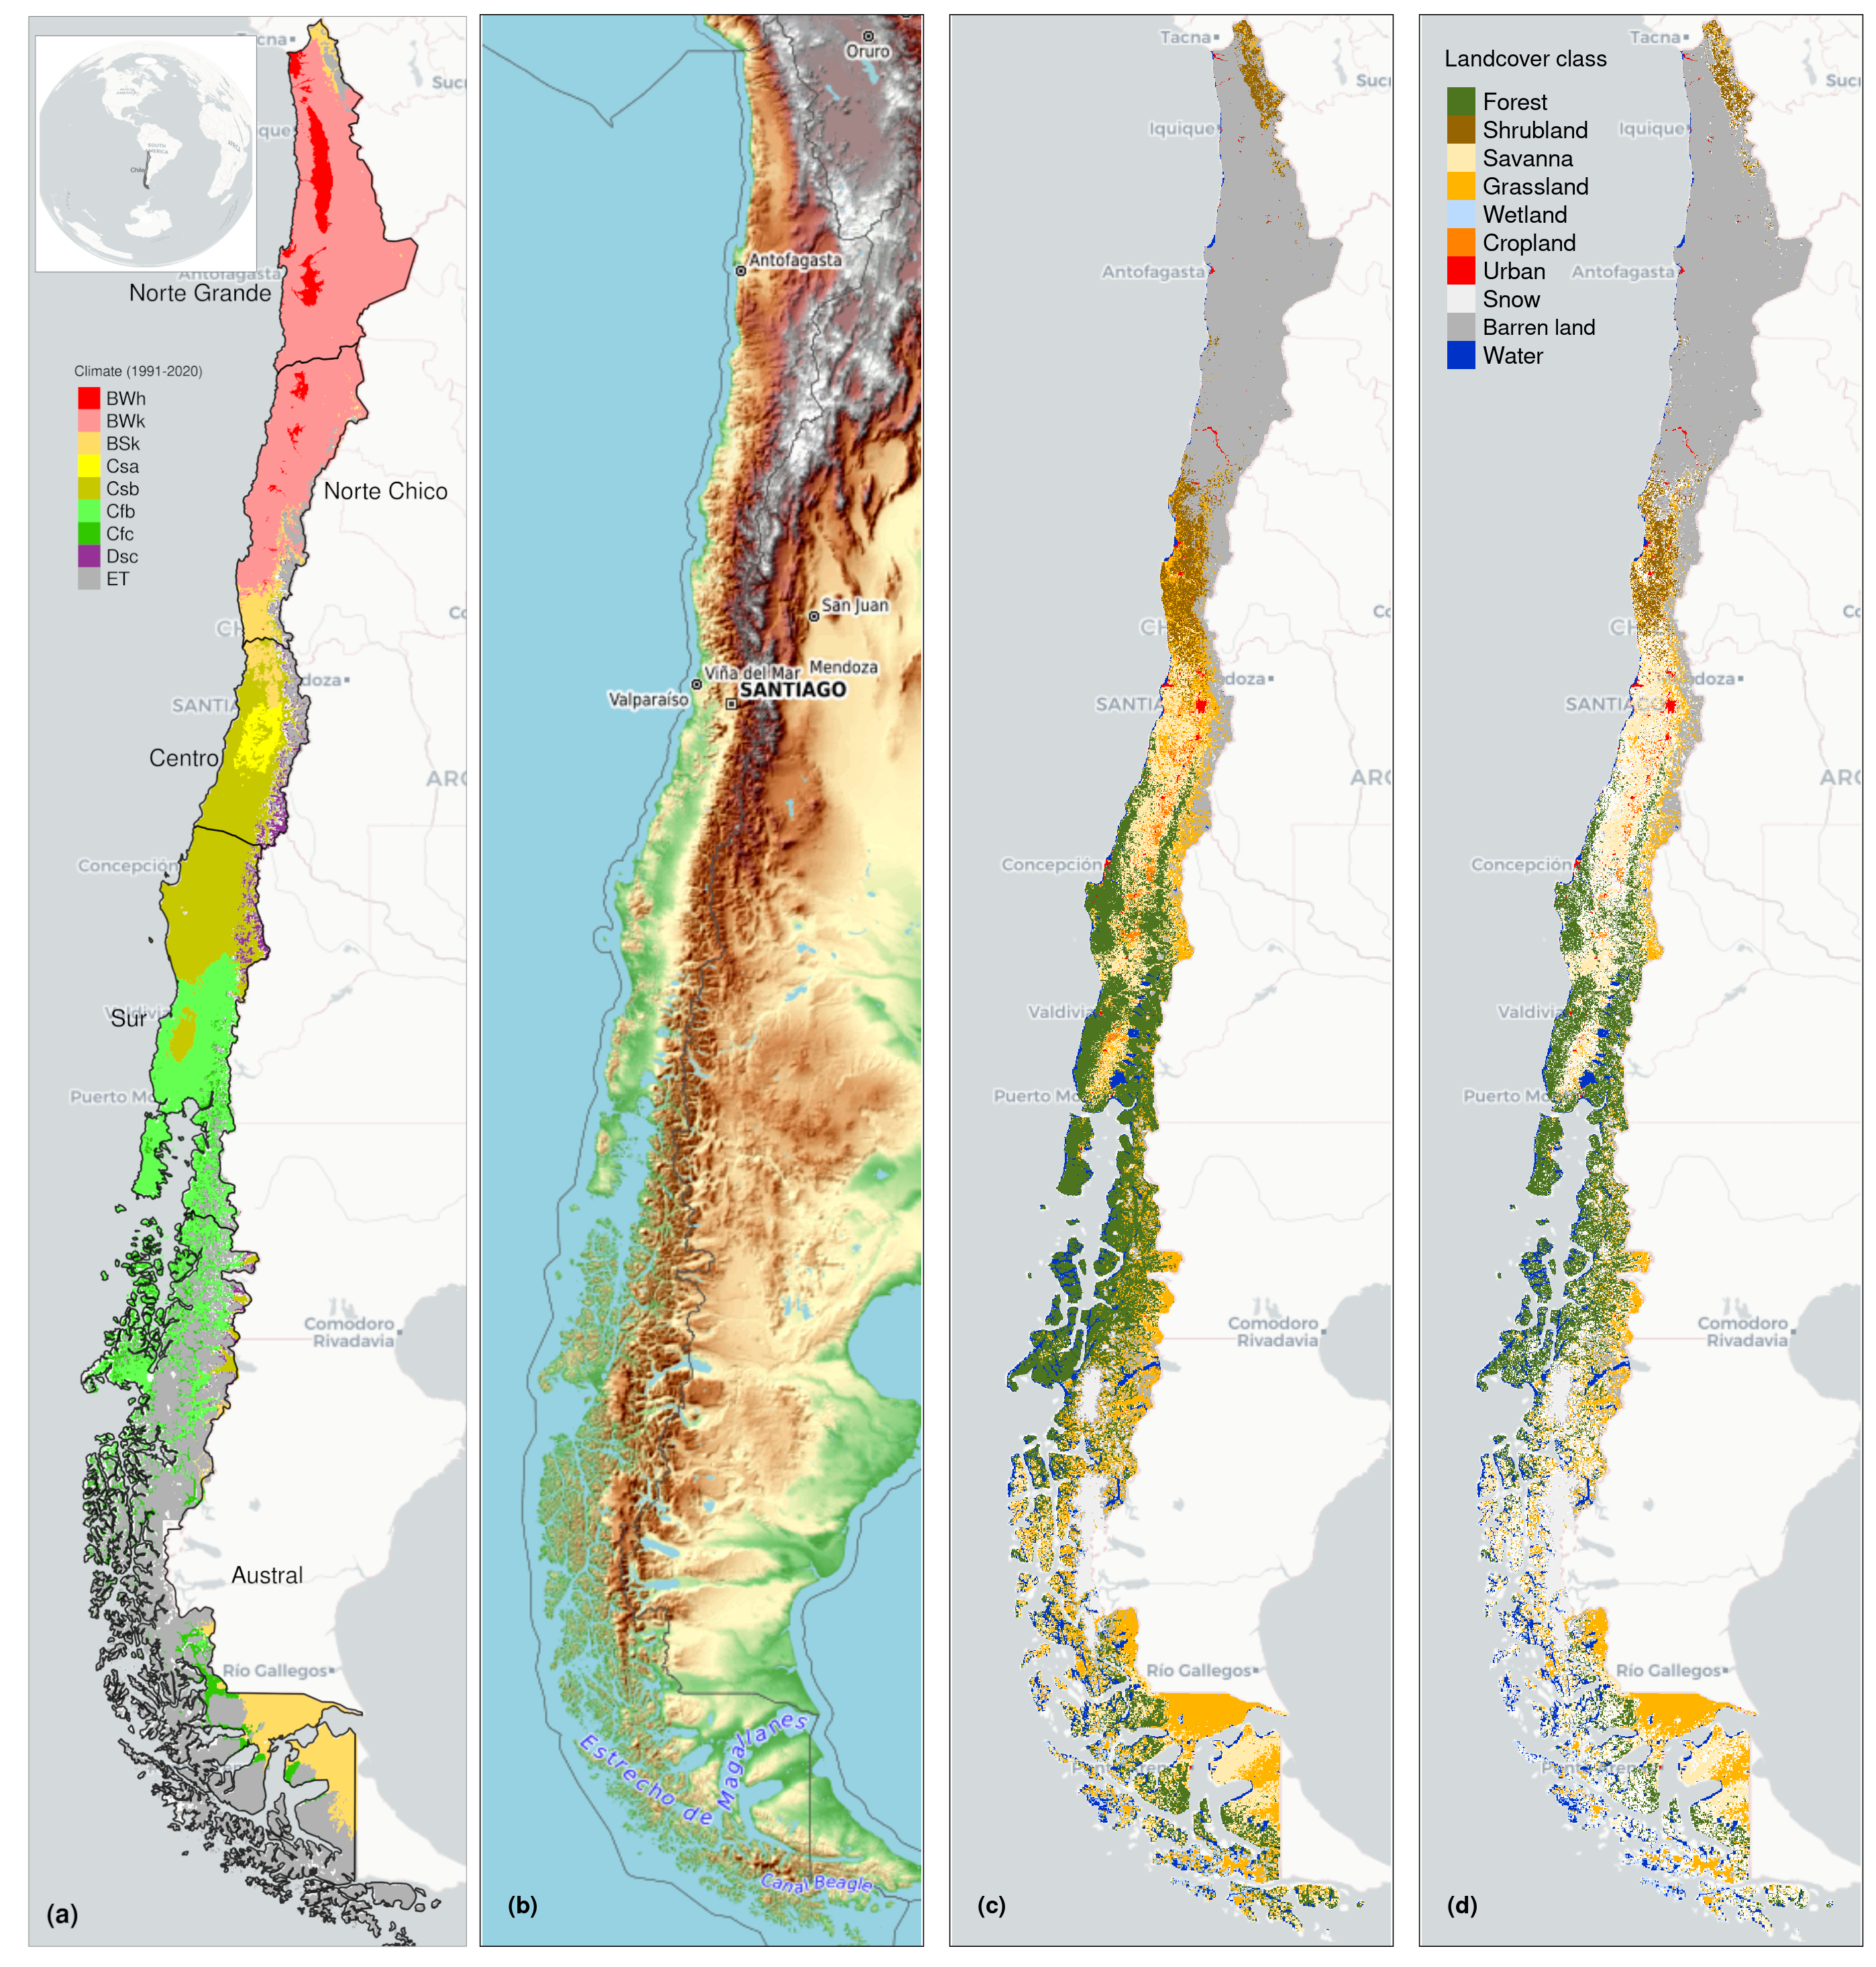
\includegraphics{../output/figs/map_study_con_landcover.png}

}

\caption{\label{fig-studyArea}(a) Chile with the Koppen-Geiger climate
classes and the five macrozones ``Norte Grande'', ``Norte Chico'',
``Centro'', ``Sur'', and ``Austral''. (b) Topography reference map. (c)
land cover classes for 2022. (d) Persistent land cover classes
(\textgreater{} 80\%) for 2001-2022}

\end{figure*}

\hypertarget{materials-and-methods}{%
\section{Materials and Methods}\label{materials-and-methods}}

\hypertarget{software-and-packages-used}{%
\subsection{Software and packages
used}\label{software-and-packages-used}}

For the downloading, processing, and analysis of the spatio-temporal
data, we used the open source software for statistical computing and
graphics, \texttt{R} \citep{R2023}. For downloading ERA5L, we used the
\texttt{\{ecmwfr\}} package \citep{Hufkens2019}. For processing raster
data, we used \texttt{\{terra\}} \citep{Hijmans2023} and
\texttt{\{stars\}} \citep{Pebesma2023}. For managing vectorial data, we
used \texttt{\{sf\}} \citep{Pebesma2018}. For the calculation of AED, we
used \texttt{\{SPEI\}} \citep{Bergueria2023}. For mapping, we use
\{tmap\} \citep{Tennekes2018}. For data analysis, the suite
\{tidyverse\} \citep{Wickham2019} was used.

\hypertarget{data}{%
\subsection{Data}\label{data}}

\hypertarget{earth-observation-data}{%
\subsubsection{Earth observation data}\label{earth-observation-data}}

For water supply and demand variables, we used ERA5L
\citep{MunozSabater2021}, a reanalys dataset that provides the evolution
of land variables since 1950. It has a spatial resolution of 0.1°,
hourly frequency, and global coverage. We selected the variables for
total precipitation, 2 meter temperature maximum and minimum, and
volumetric soil water layers between 0 and 100cm of depth (layer 1 to
layer 3). The data was downloaded using the Copernicus Climate Data
Store (CDS) Application Program Interface (API) implemented in
\texttt{\{ecmfwr\}} \citep{Hufkens2019}.

To derive a proxy for vegetation productivity, we used the product
MOD13A3 collection 6.1 from MODIS \citep{Didan2015}. It provides
vegetation indices (NDVI and EVI) at 1km of spatial resolution and
monthly frequency. The MOD13A3.061 and MCD12Q1.061 were retrieved from
the online Data Pool, courtesy of the NASA EOSDIS Land Processes
Distributed Active Archive Center (LP DAAC), USGS Earth Resources
Observation and Science (EROS) Center, Sioux Falls, South Dakota,
https://lpdaa.usgs.gov/tools/data-pool/.

\begin{table}[!ht]
\caption{Description of the earth observation data used }
\label{tab-desEOD}
\small
\centering
\begin{tabular}{p{0.13\textwidth}cp{0.3\textwidth}p{0.095\textwidth}ccc}
\hline
\multirow{1}{*}{\centering Product} & Sub-product & Variable & Spatial Resolution  & Period & Units & Short Name \\ 
\hline
\multirow{4}{*}{ERA5L} & ~ & Precipitation & \multirow{4}{*}{~0.1°} & \multirow{4}{*}{1981-2023} & mm & P \\ 
         &  & Maximum temperature & ~ & & $°C$ & $T_{max}$ \\ 
         &  & Minimum temperature & ~ & & $°C$ & $T_{min}$ \\ 
         &  & Volumetric Soil Water Content at 1m & ~ & & $m3/m3$ & SM \\ 
ERA5L* & & Atmospheric Evaporative Demand & 0.1° & 1981-2023 & mm & AED \\
        \multirow{2}{*}{MODIS} & MOD13A3.061 & Normalized Difference Vegetation Index & \multirow{2}{*}{~1 km} & 2000-2023 & ~ & NDVI \\ 
         & MCD12Q1.061 & land cover IGBP scheme & & 2001-2022 & ~ & land cover \\ 
\hline
\end{tabular}
{\raggedright *Derived from ERA5L with Eq. \ref{eq-AED}. \par}
\end{table}

\hypertarget{weather-stations}{%
\subsubsection{Weather stations}\label{weather-stations}}

We compared the ERA5L variables for monthly mean temperature, total
precipitation, and volumetric soil water content against values
retrieved by weather stations. For temperature and precipitation, we
used the weather network from the Ministry of Agriculture of Chile
(www.agromet.com) between 2015 and 2023. We used 277 stations located
throughout Chile. For soil moisture, we select a private soil network
that is owned by the agricultural enterprise Garces Fruit, which has 99
stations in Central Chile, located in cherry fruit crops. The sensors
are installed at 30, 60, and 90m and are the model Teros 12 from
MeterGroup. To avoid the effect of irrigation on soil moisture, which
ERA5L hardly captures, we used daily data for the year 2022 and the
months outside the growing season, May to September.

\hypertarget{validation-of-era5l-variables}{%
\subsubsection{Validation of ERA5L
variables}\label{validation-of-era5l-variables}}

To account for the performance of the ERA5L climatic variables regarding
the values measured by the weather stations. We selected the following
metrics:

\[MAE = \frac{1}{n}\sum |{E-S}|\] \[Bias = \frac{\sum E}{\sum S}\]
\[ubRMSE =\sqrt{\frac{\sum{ \left[ (E_i-\overline{E})-(S_i-\overline{S}) \right ] ^2}}{n}}\]

\[CC = \frac{\sum (S_i-\bar{S})(E_i-\bar{E})}{\sqrt{(Si-\bar{S})^2(E_i-\bar{E})^2}}\]

\(MAE\): mean absolute error \(bias\): bias \(ubRMSE\): unbiassed root
mean squared error \(CC\): coefficient of correlation \(S\): value of
the variable measure by the weather station \(E\): value of the variable
measure by ERA5L

\hypertarget{drought-indices}{%
\subsection{Drought Indices}\label{drought-indices}}

\hypertarget{atmospheric-evaporative-demand-aed}{%
\subsubsection{Atmospheric Evaporative Demand
(AED)}\label{atmospheric-evaporative-demand-aed}}

For the indices EDDI and SPEI that use water demand, first we have to
calculate the AED. For this, we used the method of Hargreaves
\citep{Hargreaves1994, Hargreaves1985}:

\begin{equation}\protect\hypertarget{eq-AED}{}{AED = 0.0023\cdot Ra\cdot (T+17.8)\cdot (T_{max}-T_{min})^{0.5}}\label{eq-AED}\end{equation}

where \(Ra\) \((MJ\,m^2\, day^{-1})\) is extraterrestrial radiation;
\(T\), \(T_{max}\), and \(T_{min}\) are mean, maximum, and minimum
temperature \((°C)\). We calculate the centroid coordinates per pixel
and use the latitude to estimate \(Ra\).

We chose the method of Hargreaves to estimate AED because of its
simplicity, which only requires temperatures and extrarrestrial
radiation. Also, it has been recommended over other methods when the use
of several climatic variables is limited \citep{Vicente-Serrano2014}.

\hypertarget{non-parametric-calculation-of-drought-indices}{%
\subsubsection{Non-parametric calculation of drought
indices}\label{non-parametric-calculation-of-drought-indices}}

We derived the drought indices of water supply and demand, soil moisture
from the ERA5L dataset, and vegetation from the MODIS product, all at
monthly frequency.

To evaluate water demand, we chose the \(EDDI\)
\citep{Hobbins2016, McEvoy2016} index, which uses the \(AED\). We used
the SPI \citep{Mckee1993}, a drought monitoring index that the World
Meteorological Organization (WMO) recommends. We calculated the SPEI,
which used a balance between \(P\) and \(AED\), in this case, an
auxiliary variable \(D = P-AED\) is used. In this study, we used the
\(SSI\) (standardized soil moisture index at 1 m)
\citep{Hao2013, AghaKouchak2014}, which uses soil moisture at 1m depth.
Finally, for the proxy of productivity, \(zcNDVI\), we used the NDVI.
Before using the NDVI, it was smoothed using a locally weighted
polynomial regression, following the procedure described in
\citet{Zambrano2018} and \citet{Zambrano2016}.

All the indices are multi-scalar and were calculated for time scales of
1, 3, 6, 12, 24, and 36 months, except for zcNDVI, which was calculated
for 6 months. The goal is to be able to evaluate short- and long-term
droughts in water demand and supply and soil moisture. This is
particularly important for central Chile because it has suffered from a
prolonged decrease in precipitation for more than 12 years
\citep{Garreaud2020, Boisier2018, Garreaud2017}.

To calculate the drought indices, first we must calculate the
accumulation of the variable. In this case, for generalization purposes,
we will use \(V\), referring to \(P\), \(AED\), \(D\), \(NDVI\), and
\(SM\) (Table \ref{tab-desEOD}). We cumulated each \(V\) over the time
series of \(n\) values, and for the time scales \(s\):

\begin{equation}\protect\hypertarget{eq-sumvar}{}{A_{si} = \sum_{i=n-s-i+2}^{n-i+1} V_i\,\, \forall\, i\geq n-s+1  }\label{eq-sumvar}\end{equation}

It corresponds to a moving window (convolution) that sums the variable
for \(s\) starting for the last month \(n\) until the month, which could
sum for \(s\) months (n-s+1). Once the variable is cumulated over time
for the scale \(s\), we used a nonparametric approach following
\citet{Hobbins2016} to derive the drought indices. Thus, the empirically
derived probabilities are obtained through an inverse normal
approximation \citep{Abramowitz1968}. Then, we used the empirical Tukey
plotting position \citep{Wilks2011} over \(A_i\) to derive the
\(P(A_i)\) probabilities across a period of interest:

\begin{equation}\protect\hypertarget{eq-probPai}{}{P(A_i) = \frac{i-0.33}{n+0.33'}}\label{eq-probPai}\end{equation}

The drought indices \(SPI\), \(SPEI\), \(EDDI\), \(SSI\), and \(zcNDVI\)
are obtained following the inverse normal approximation:

\begin{equation}\protect\hypertarget{eq-DI}{}{DI(A_i) = W - \frac{C_0+C_1\cdot W + c_2 \cdot W^2}{1+d_1\cdot W +d_2\cdot W^2 +d_3\cdot W^3}}\label{eq-DI}\end{equation}

\(DI\) is referring to the drought index calculated for the variable
\(V\). The values for the constats are: \(C_0 = 2.515517\),
\(C_1 = 0.802853\), \(C_2 = 0.010328\), \(d_1 = 1.432788\),
\(d_2 = 0.189269\), and \(d3 = 0.001308\). For \(P(A) \leq 0.5\),
W=\(\sqrt{-2\cdot ln(P(A_i))}\) , and for \(P(A_i) > 0.5\), replace
\(P(A_i)\) with \(1-P(A_i)\) and reverse the sign of \(DI(A_i)\).

\hypertarget{sec-methods_lulc}{%
\subsection{LULC change for 2001-2022 and its relation with water supply
and demand, and soil moisture}\label{sec-methods_lulc}}

\hypertarget{land-cover-macroclasess-and-validation}{%
\subsubsection{Land cover macroclasess and
validation}\label{land-cover-macroclasess-and-validation}}

To analyze the LULCC, we use the IGBP scheme from the MCD12Q1 collection
6.1 from MODIS. This product has a yearly frequency from 2001 to 2022.
The IGBP defines 17 classes; from these, we regrouped into ten
macroclasses, as follows: classes 1-4 to forest, 5-7 to schrublands, 8-9
to savannas, 10 as grasslands, 11 as wetlands, 12 and 14 to croplands,
13 as urban, 15 as snow and ice, 16 as barren, and 17 to water bodies.
Thus, we have a land cover raster time series with the ten classes for
2001 and 2023.

To validate the land cover obtained, we compare the macroclasses with
the ones of a more detailed land cover map made by \citet{Zhao2016} for
Chile with samples acquired in the years 2013--2014 (LCChile). The later
has a spatial resolution of 30 m and three levels of defined classes;
from those, we used level 1, which fits with the macroclasses land
cover. We chose the years 2013 (IGBP2013) and 2014 (IGBP2014) from land
cover macrolcasses to validate with LCChile.

We follow the next procedure:

\begin{enumerate}
\def\labelenumi{\roman{enumi})}
\tightlist
\item
  resampled LCChile to the spatial resolution (500m) of the land cover
  macroclasses using the nearest neighbor method,
\item
  took a random sample of 1000 points within continental Chile and
  extracted the classes that fell within each point for LCChile,
  IGBP2013, and IGBP2014; we considered the point extracted from LCChile
  as the truth and the values from the other two years as predictions.
\item
  calculate a confusion matrix with the classes extracted from the 1000
  points for LCChile, IGBP2013, and IGBP2014. Calculate the performance
  metrics of accuracy and F1.
\end{enumerate}

\[Accuracy = \frac{TP+TN}{TP+TN+FP+FN}=\frac{correct\,\, classifications}{all\,\, classifications}\]
\[F1=\frac{2\cdot TP}{2\cdot TP + FP +FN}\] where \(TP\) and \(FN\)
refer to true positive and false negative, correctly classified classes;
\(TN\) and \(FP\) to true negative and false positive, wrongly
classified classes.

\hypertarget{land-cover-persistence-mask-2001-2022}{%
\subsubsection{Land cover persistence mask
2001-2022}\label{land-cover-persistence-mask-2001-2022}}

Climate, vegetation development, seasonality, and changes in vegetation
type all have an impact on the time series of NDVI. In this study, we
want to examine the variation in vegetation productivity across various
land cover types and how water demand, water supply, and soil moisture
affect it. In order to avoid changes due to a change in the land cover
type that will wrongly impact NDVI, we will develop a persistence mask
for land cover for 2001--2023. Thereby, we reduce an important source of
variation on a regional scale.

Therefore, we generated a raster mask for IGBP MODIS per pixel using
macroclasses that remain constant for at least 80\% of the years
(2001--2022). This enables us to identify regions where the land cover
of the macroclasses has remained constant.

\hypertarget{land-cover-trend-and-drought-indices}{%
\subsubsection{Land cover trend and drought
indices}\label{land-cover-trend-and-drought-indices}}

We calculated the surface occupied per land cover class into the five
macrozones (``Norte Grande'' to ``Austral'') per year for 2001--2023.
After that, we calculated the trend's change in surface; we used the
Sen' slope \citep{Sen1968} based on Mann-Kendall \citep{Kendall1975}.
This way, we obtain a matrix of trends of 5 x 5 (macrozones x land
cover). The aim is to later explore if the trend in land cover classes
is associated with a trend in the drought indices. For this, we will use
the techniques of regresion and regularization of Lasso
\citep{Tibshirani2010} and Ridge \citep{Hoerl1970}. Also, we will test
random forests for this purpose \citep{Ho1995}. We will choose the trend
of land cover surface per macroclass and macrozone as the response
variable and the trend of the drought indices (SPI, SPEI, EDDI, and SSI
for time scales 1, 3, 6, 12, 24, and 36 months) as the predictor
variables. With this analysis, we expect to gather insights regarding
whether there is a pattern of climatic influence along Chile or if what
is happening in Central Chile has to do with more localized climatic
conditions.

\hypertarget{trend-of-drought-indices-for-water-demand-and-supply-soil-moisture-and-vegetation-productivity}{%
\subsection{Trend of drought indices for water demand and supply, soil
moisture, and vegetation
productivity}\label{trend-of-drought-indices-for-water-demand-and-supply-soil-moisture-and-vegetation-productivity}}

\hypertarget{mann-kendall-and-sens-slope}{%
\subsubsection{Mann-Kendall and Sen's
slope}\label{mann-kendall-and-sens-slope}}

To estimate if there are significant positive or negative trends for the
drought indices, we used the non-parametric test of Mann-Kendall
\citep{Kendall1975}. To determine the magnitude of the trend, we used
Sen's slope \citep{Sen1968}. Some of the advantages of applying this
methodology are that the Sen's slope is not affected by outliers as
regular regression does, and it is a non-paramteric method that is not
affected by the distribution of the data. We applied both to the six
time scales from 1981 to 2023 (monthly frequency) and the indices SPI,
EDDI, SPEI, and SSI. In the case of zcNDVI (six months) was for 2000 to
2023. Thus, we have 31 trends. Also, we extracted the trend aggregated
by macrozone and land cover class, obtaining a table of 31x5x5 (drought
indices trends x macrozone x land cover class). We will use this data in
Section~\ref{sec-methods_lulc} to analyze if there is a strong
relationship between the trends of drought indices and land cover
surface within continental Chile.

\hypertarget{trend-in-vegetation-productivity-without-land-cover-change}{%
\subsubsection{Trend in vegetation productivity without land cover
change}\label{trend-in-vegetation-productivity-without-land-cover-change}}

\citet{Vicente-Serrano2021} made a global analysis of the drought's
severity trend using SPI, SPEI, and the Standardized Evapotranspiration
Deficit Index (SEDI; \citet{Vicente-Serrano2018}) to evaluate AED. They
indicate that the increase in hydrological drought has been due to
anthropogenic effects rather than climate change. This is because the
global increase in AED did not explain the change in the spatial pattern
of the hydrological drought. Also, they state that \emph{``the increase
in hydrological droughts has been primarily observed in regions with
high water demand and land cover change''}. We will contrast this
hypothesis with what is occurring in Chile. To achieve this, we will use
the land cover class type that remains more than 80\% of types for
2001--2022 to evaluate the trend on zcNDVI and use this as a mask where
there are low changes.

\hypertarget{impact-for-water-supply-and-demand-and-soil-moisture-in-vegetation-productivity-within-land-cover-types}{%
\subsection{Impact for water supply and demand, and soil moisture in
vegetation productivity within land cover
types}\label{impact-for-water-supply-and-demand-and-soil-moisture-in-vegetation-productivity-within-land-cover-types}}

We analyze the drought indices of water demand and supply and soil
moisture against vegetation to address: i) if short- or long-term time
scales are most important in impacting vegetation through Chile; and ii)
the strength of the correlation for the variable and the time scale.
Then, we will summarize for each land cover class and macrozone. Thus,
we will be able to advance in understanding how climate is affecting
vegetation, considering the impact on the five macroclasses of
vegetation: forest, cropland, grassland, savanna, and shrubland.

An analysis is conducted on the linear correlation between the indices
SPI, SPEI, EDDI, and SSI over time periods of 1, 3, 6, 12, 24, and 36
months, and zcNDVI. The objective is to determine the impact of soil
moisture and water demand and supply on vegetation productivity. We
implemented a methodology similar to that of \citet{Meroni2016} when
comparing the SPI for meteorological drought to the cumulative FAPAR
(Fraction of Absorbed Photosynthetically Active Radiation), which served
as an indicator for vegetation productivity. A pixel-to-pixel linear
correlation analysis was performed for each index. To begin, the Pearson
coefficient of correlation is computed for each of the six time scales.
A significant time scale is identified as the one that attains the
highest correlation (p \textless{} 0.05). Subsequently, the Pearson
correlation coefficient corresponding to the time scales at which the
value peaked was extracted. As a result, for each index, we generated
two raster maps: one containing the time scales and the other the
correlation value.

\hypertarget{results}{%
\section{Results}\label{results}}

\hypertarget{data-1}{%
\subsection{Data}\label{data-1}}

\hypertarget{validation-of-era5l-variables-1}{%
\subsubsection{Validation of ERA5L
variables}\label{validation-of-era5l-variables-1}}

The average metrics of performance of ERA5L over the 266 weather
stations were in the case of monthly temperature: \(ubRMSE=1.06\,°C\),
\(MAE=1.131\,°C\), and \(CC=0.963\), showing a good agreement, low
error, and low overestimation. For cumulative monthly precipitation,
\(MAE=28.1\,mm\), \(bias=1.93\), and \(CC=0.845\), showing a high
correlation and a 93\% bias and being overestimated by ERA5L. In the
case of the 97 soil moisture stations, we averaged for the three depths
(30, 60, and 90m) and then compared it with volumetric water content at
1m derived from ERA5L. For this case, we made a daily comparison, having
a \(CC=0.71\), \(RMSE=0.174\,m^3m^{-3}\), \(MAE=0.167\,m^3m^{-3}\), and
\(bias=1.74\). The ERA5 soil moisture overestimate is 74\%, but it has a
kind of good correlation. For more detailed information, consult the
supplementary material (SSX).

\hypertarget{lulc-change-for-2001-2022-and-its-relation-with-water-supply-and-demand-and-soil-moisture}{%
\subsection{LULC change for 2001-2022 and its relation with water supply
and demand, and soil
moisture}\label{lulc-change-for-2001-2022-and-its-relation-with-water-supply-and-demand-and-soil-moisture}}

\hypertarget{land-cover-macroclasess-and-validation-1}{%
\subsubsection{Land cover macroclasess and
validation}\label{land-cover-macroclasess-and-validation-1}}

For vegetation, we obtained and use hereafter five macroclasses of land
cover from IGBP MODIS: forest, shrubland, savanna, grassland, and
croplands. Figure~\ref{fig-studyArea} c shows the spatial distribution
of the macroclasses through Chile for the year 2022. The validation of
IGBP2013 and IGBP2014 with LCChile reached near the same metrics of
performance, having an accuracy of \textasciitilde0.82 and a F1 score of
\textasciitilde0.66 (see SS1).

\hypertarget{sec-persistence_mask}{%
\subsubsection{Land cover persistence mask
2001-2022}\label{sec-persistence_mask}}

Figure~\ref{fig-studyArea} d, shows the macroclasses of land cover
persistance (80\%) during 2021-2022, respectively
(\ref{tab-landcoverSurf}). Within continental Chile, forest is the
vegetation type with the highest surface area at 135,00 \(km^2\),
followed by grassland (73,176 \(km^2\)), savanna (54,410 \(km^2\)),
shrubland (24,959 \(km^2\)), and cropland (3,100 \(km^2\)) (Table
\ref{tab-landcoverSurf}). The macrozones with major LULCC for 2001--2022
were ``Centro,'' ``Sur,'' and ``Austral'' with 36\%, 31\%, and 34\%,
respectively (Figure~\ref{fig-studyArea} and Table
\ref{tab-landcoverTrend}); of its surface that changes the type of land
cover. Figure~\ref{fig-LCprop} shows the summary of the proportion of
surface per land cover class and macrozone, derived from the persistance
mask over continental Chile.

\begin{table}[!ht]
\caption{Surface of the land cover class that persist during 2001-2022}
\label{tab-landcoverSurf}
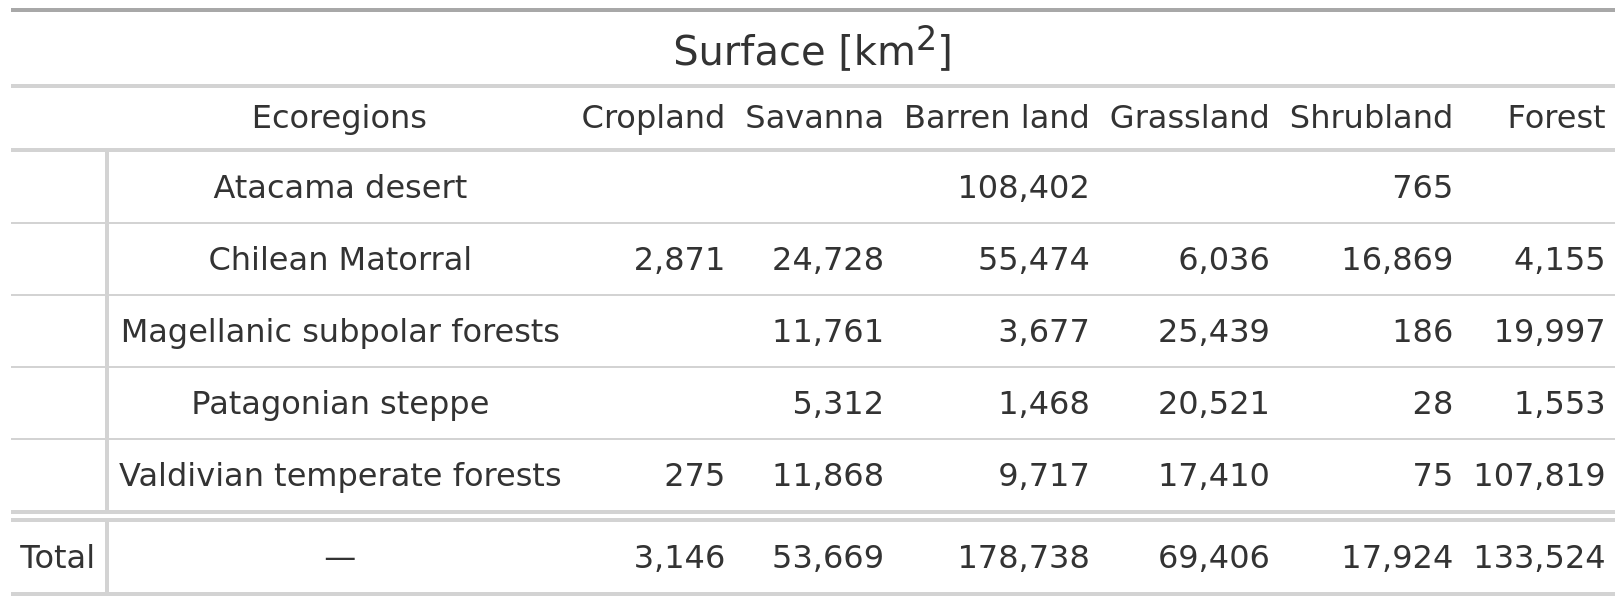
\includegraphics[width = .5\textwidth]{../output/figs/table_surface_landcover_macrozone.png}
\end{table}

\begin{figure}[!ht]

{\centering 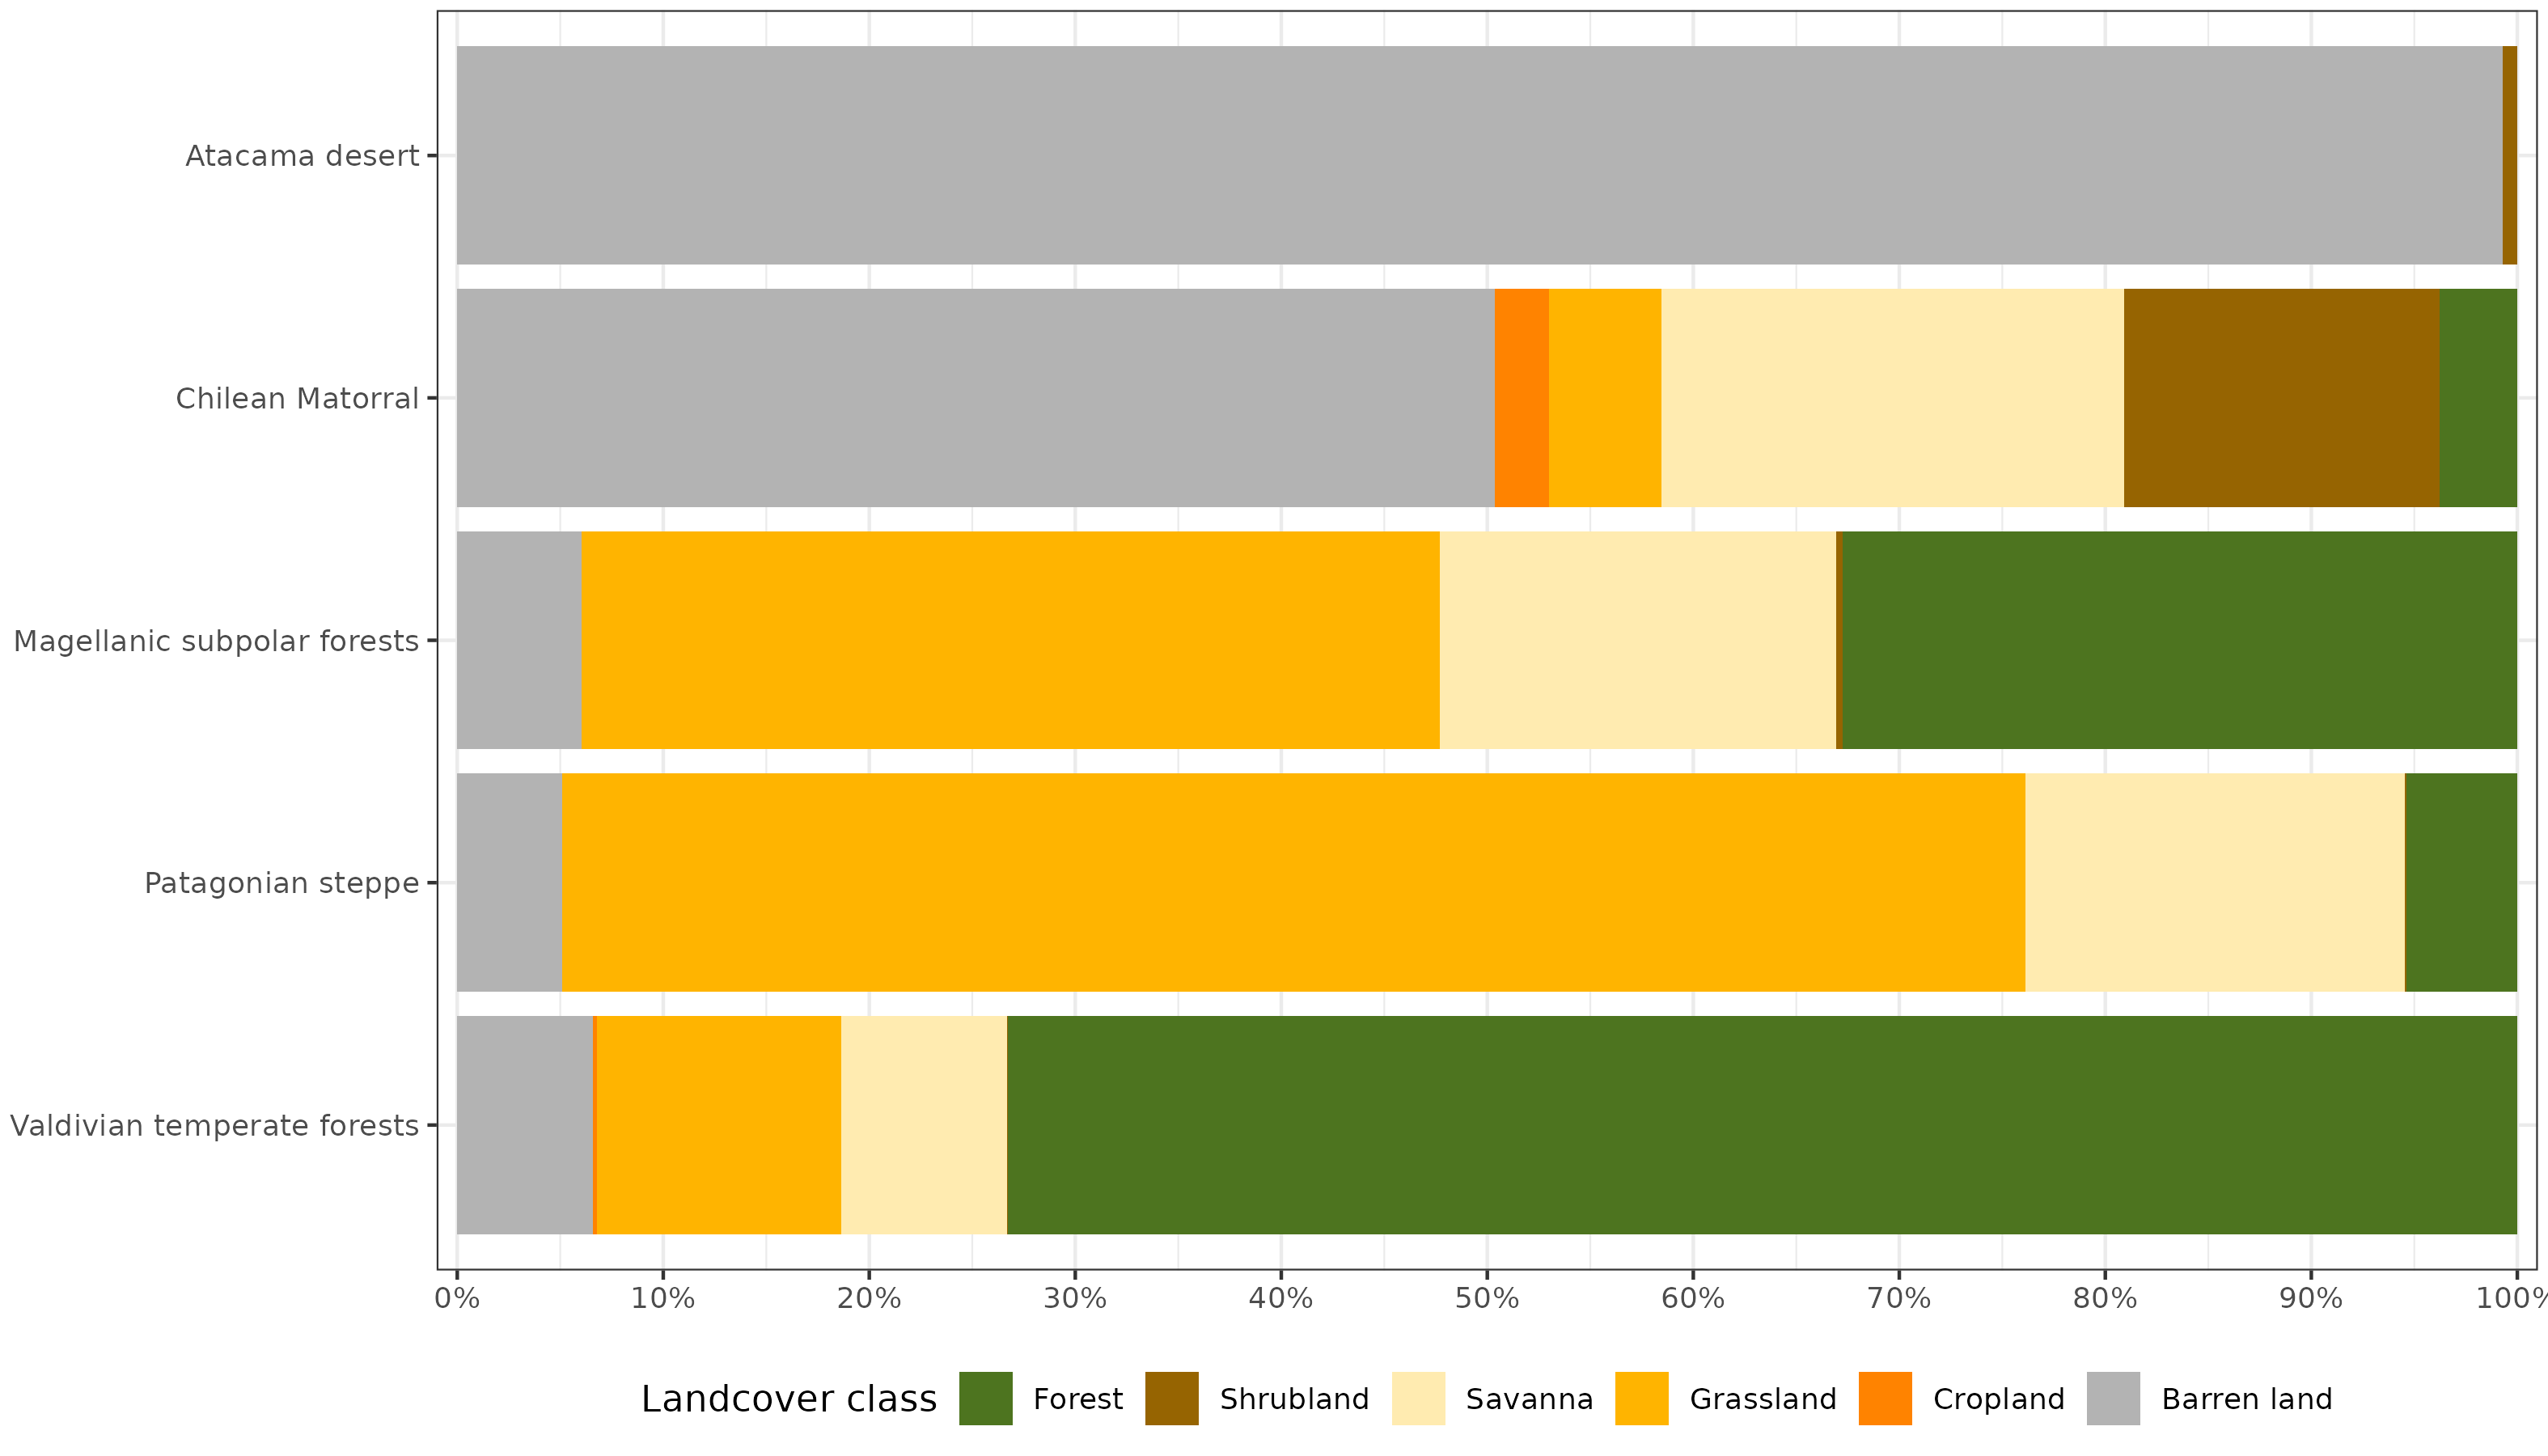
\includegraphics{../output/figs/LC_pers80_per_macrozone.png}

}

\caption{\label{fig-LCprop}Proportion of land cover class from the
persistent land cover for 2001-2022 (\textgreater80\%) per macrozone}

\end{figure}

\hypertarget{land-cover-trend-and-drought-indices-1}{%
\subsubsection{Land cover trend and drought
indices}\label{land-cover-trend-and-drought-indices-1}}

\begin{table}[!ht]
\caption{The value of Sen's slope trend next to the time-series plot of surface per land cover class (IGBP MCD12Q1.016) for 2001–2022 through Central Chile. Values of zero indicate that there was not a significant trend. Red dots on the plots indicate the maximum and minimum values of surface.}
\label{tab-landcoverTrend}
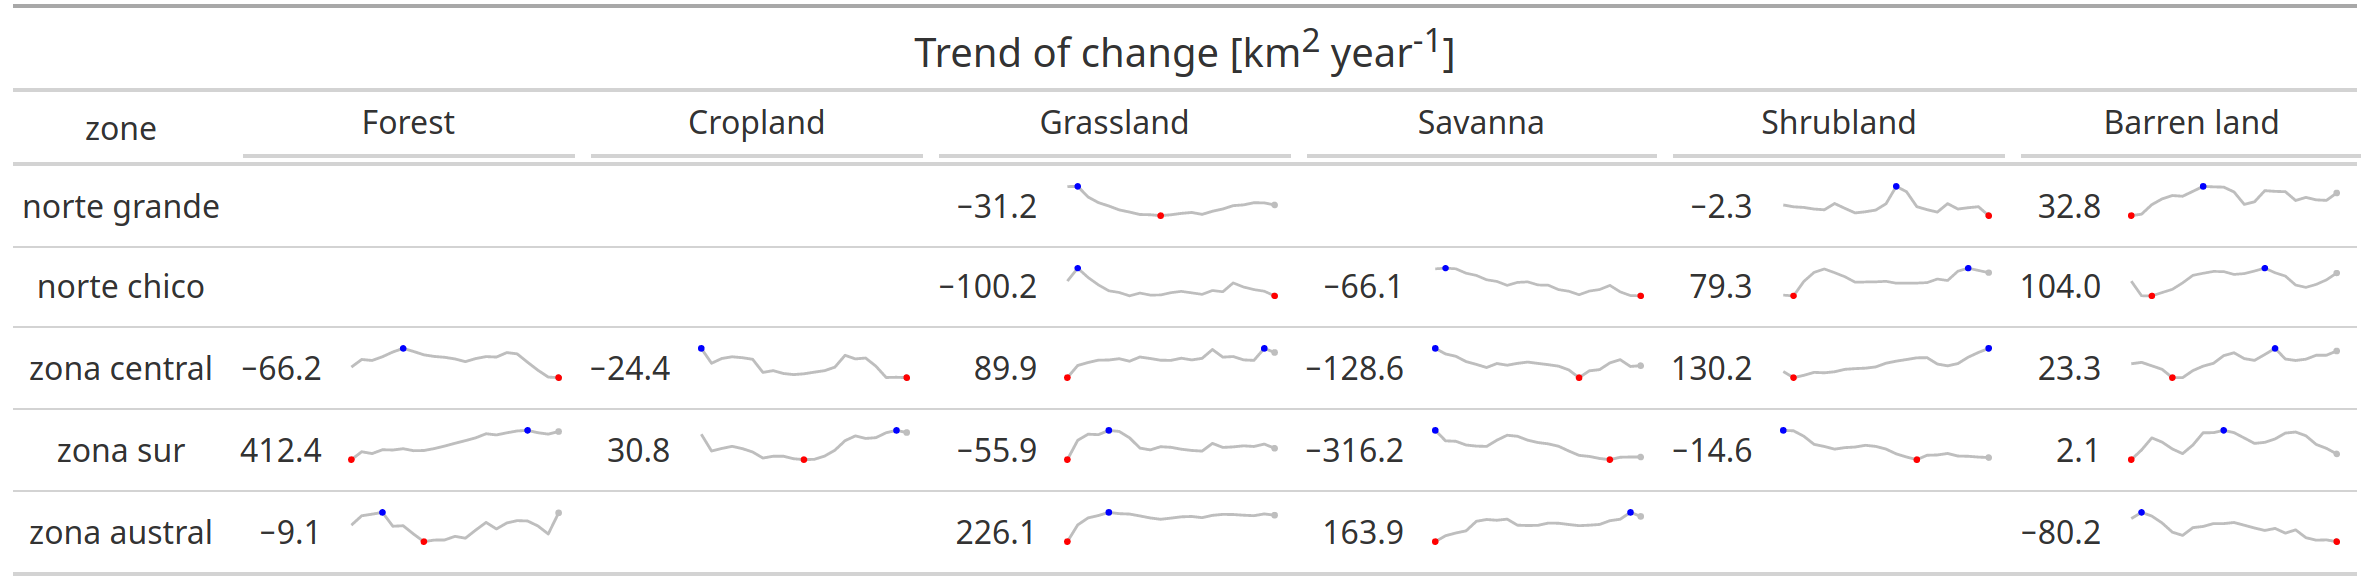
\includegraphics[]{../output/figs/table_var_landcover_macro.png}
\end{table}

The ``Norte Chico'' shows an increase in barrend land of 111
\(km^2 year^{-1}\) and a reduction in the class savanna of 70
\(km^2 year^{-1}\). In the ``Centro'' and ``Sur,'' there are changes in
the Chilean matorral, with an important reduction in savanna (136 to 318
\(km^2 yr^{-1}\)), and an increase in shrubland and grassland. Showing a
change for more dense vegetation types. It appears to be a shift in the
area of cropland from the ``Centro'' to the ``Sur.'' Also, there is a
high increase in forest (397 \(km^2 yr^{-1}\)) in the ``Sur,'' replacing
the savanna lost.

Further, we want to address whether the trend in land cover change for
2001--2023 is associated with trends in drought indices of water demand
and supply and/or soil moisture for macrozone and land cover
macroclasses. From the three methods tested, Ridge, Lasso, and Random
Forest, neither gives significant results regarding whether the trend in
a drought index for any time scale explains the trend in land cover
change. Nevertheless, in ``Norte Chico'' and ``Centro,'' there is a
decrease in croplands and savanna and an increase in barren land, which
is associated with the variation in drought indices. Mainly for a
decrease in water supply (SPI and SSI) and an increase in water demand
(EDDI). However, due to the high variability from north to south in
Chile, the climatic conditions (arid, semi-arid, and humid), and the
land cover type, we believe that only in those zones could the LULCC be
driven to some degree by drought.

\hypertarget{trend-of-drought-indices-for-water-demand-and-supply-soil-moisture-and-vegetation-productivity-1}{%
\subsection{Trend of drought indices for water demand and supply, soil
moisture, and vegetation
productivity}\label{trend-of-drought-indices-for-water-demand-and-supply-soil-moisture-and-vegetation-productivity-1}}

\begin{figure}[!ht]

{\centering 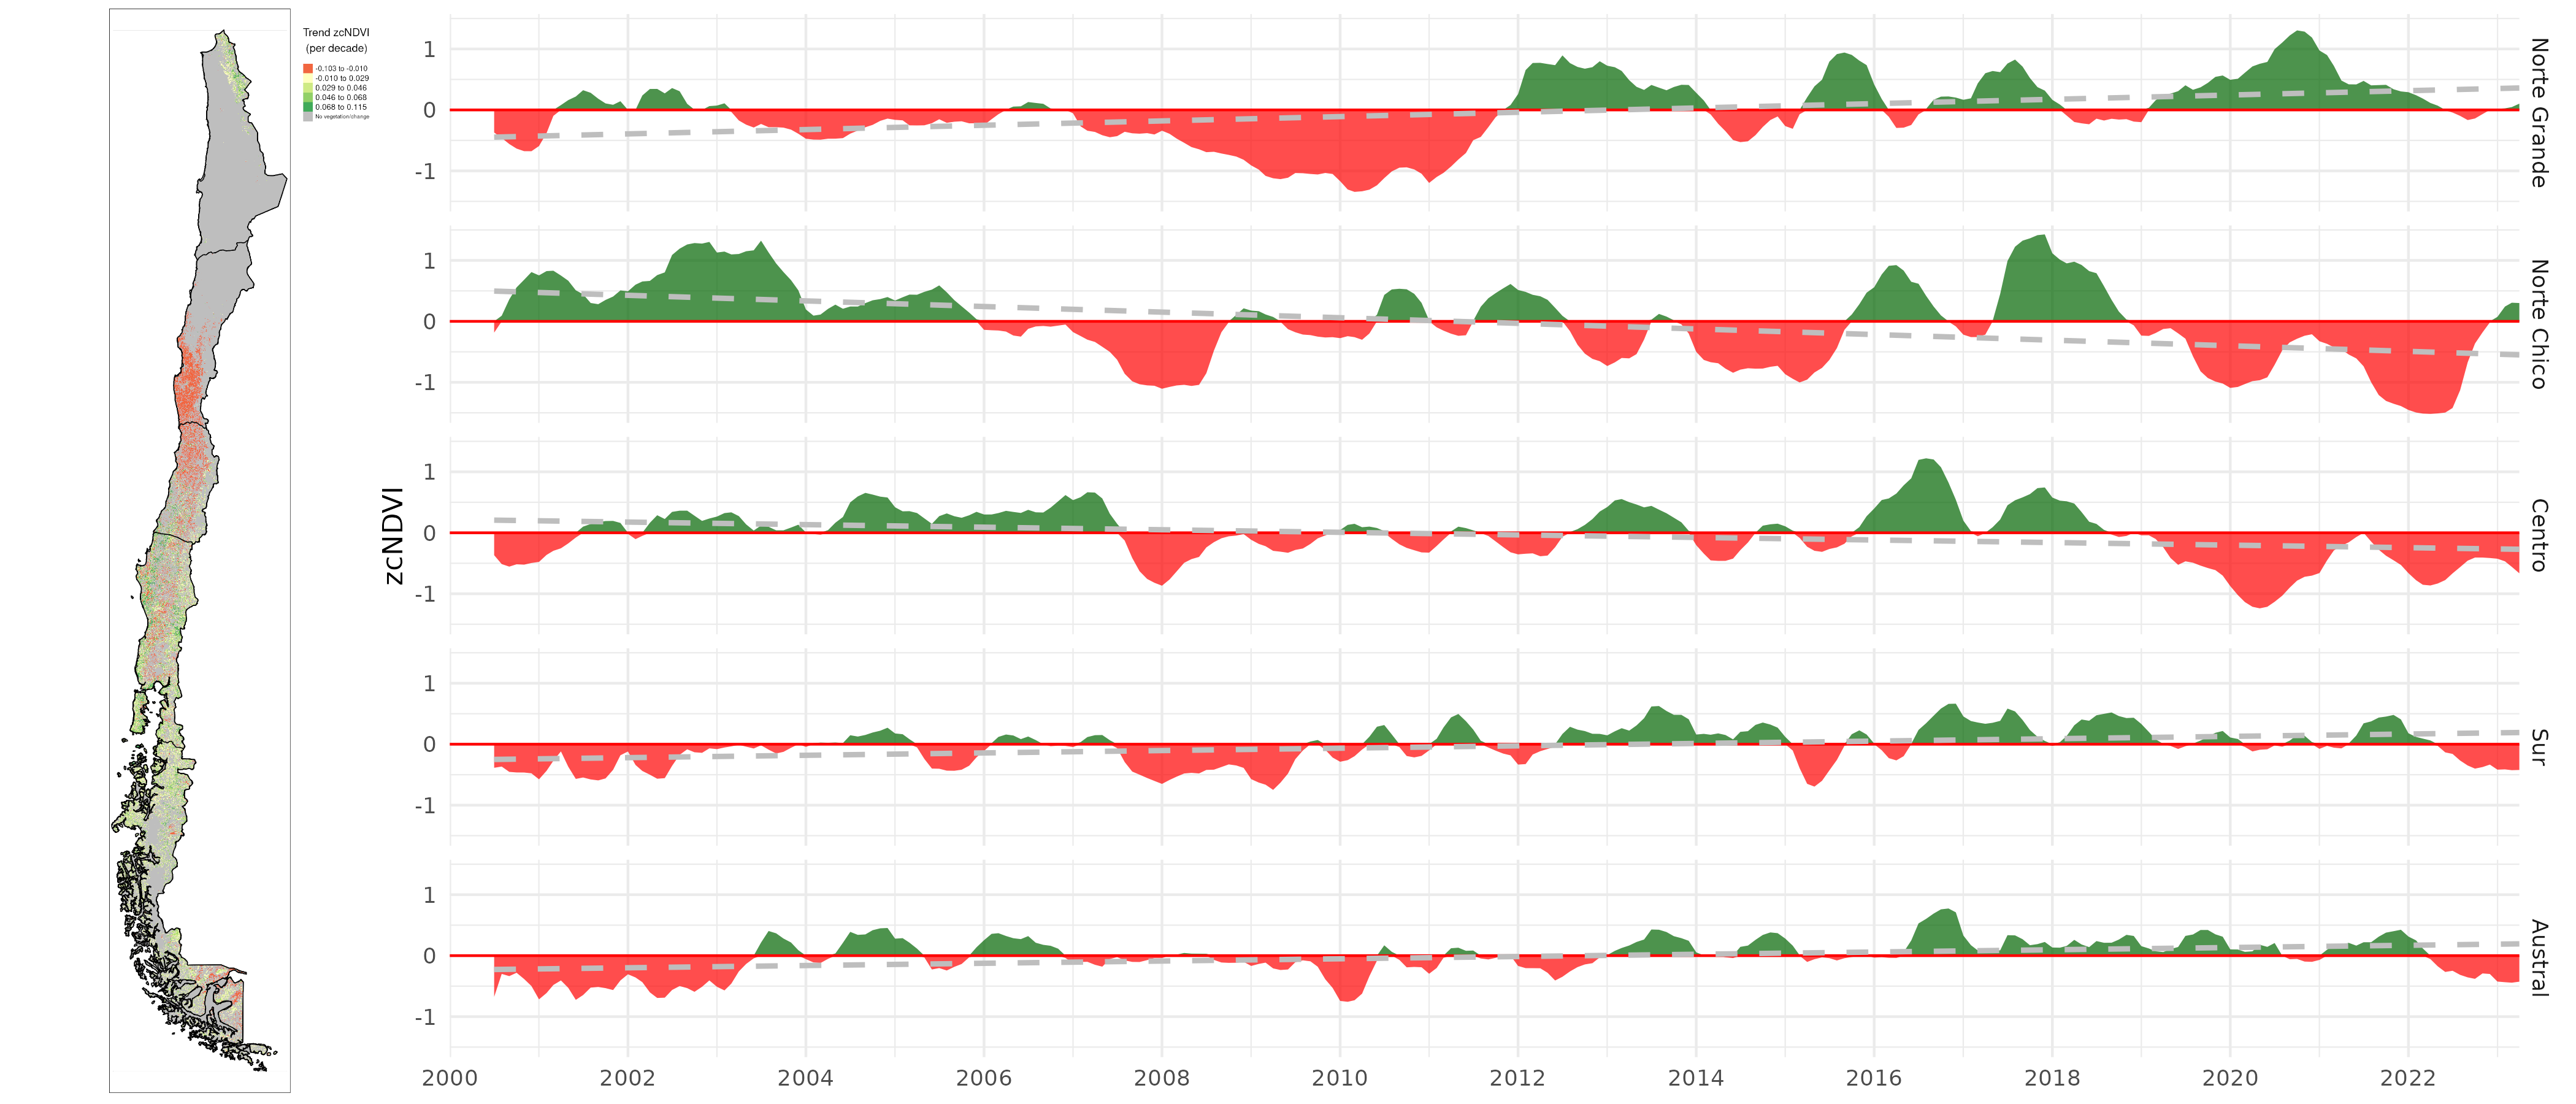
\includegraphics{../output/figs/temporal_variation_zcNDVI6_macrozonas_con_mapa.png}

}

\caption{\label{fig-zcNDVI_var}(a) Map of the linear trend of the index
zcNDVI-6 for 2001--2023. Greener colors indicate a positive trend; reder
colors correspond to a negative trend and a decrease in vegetation
productivity. Grey colors indicate either no vegetation or a change in
land cover type for 2001--2022. (b) Temporal variation of zcNDVI-6
aggregated at macrozone level within continental Chile. Each horizontal
panel corresponds to a macrozone from `Norte Grande' to `Austral'.}

\end{figure}

In ``Norte Grande,'' vegetation productivity, as per the z-index,
exhibits a yearly increase of 0.02 in the five land cover macroclasses,
with respect to grassland and shrubland categories. There is a negative
trend in ``Norte Chico'' with -0.04 and ``Centro'' with -0.02 per
decade. In the ``Norte Chico,'' savanna (-0.05) has the lowest trend,
and the rest of the types are around -0.04. In ``Centro,'' shrubland
reaches -0.06, grassland -0.05, and croplands and savanna -0.01 per
decade. This could be associated either with a reduction in vegetation
surface, a decrease in biomass, or browning \citep{Miranda2023}.
Vegetation reached its lowest values since the year 2019, reaching an
extreme condition in early 2020 and 2022 in the ``Norte Chico'' and
Centro'' (Mega Drought). The ``Sur'' and ``Austral'' show a positive
trend of around 0.016 per decade (Figure~\ref{fig-zcNDVI_var}). Despite
the croplands suffering from drought just as badly as the native
vegetation in ``Norte Chico,'' the Chilean matorral \citep{Fuentes2021}
appears to be the region most affected by a negative trend in vegetation
productivity.

\begin{figure}[!ht]

{\centering 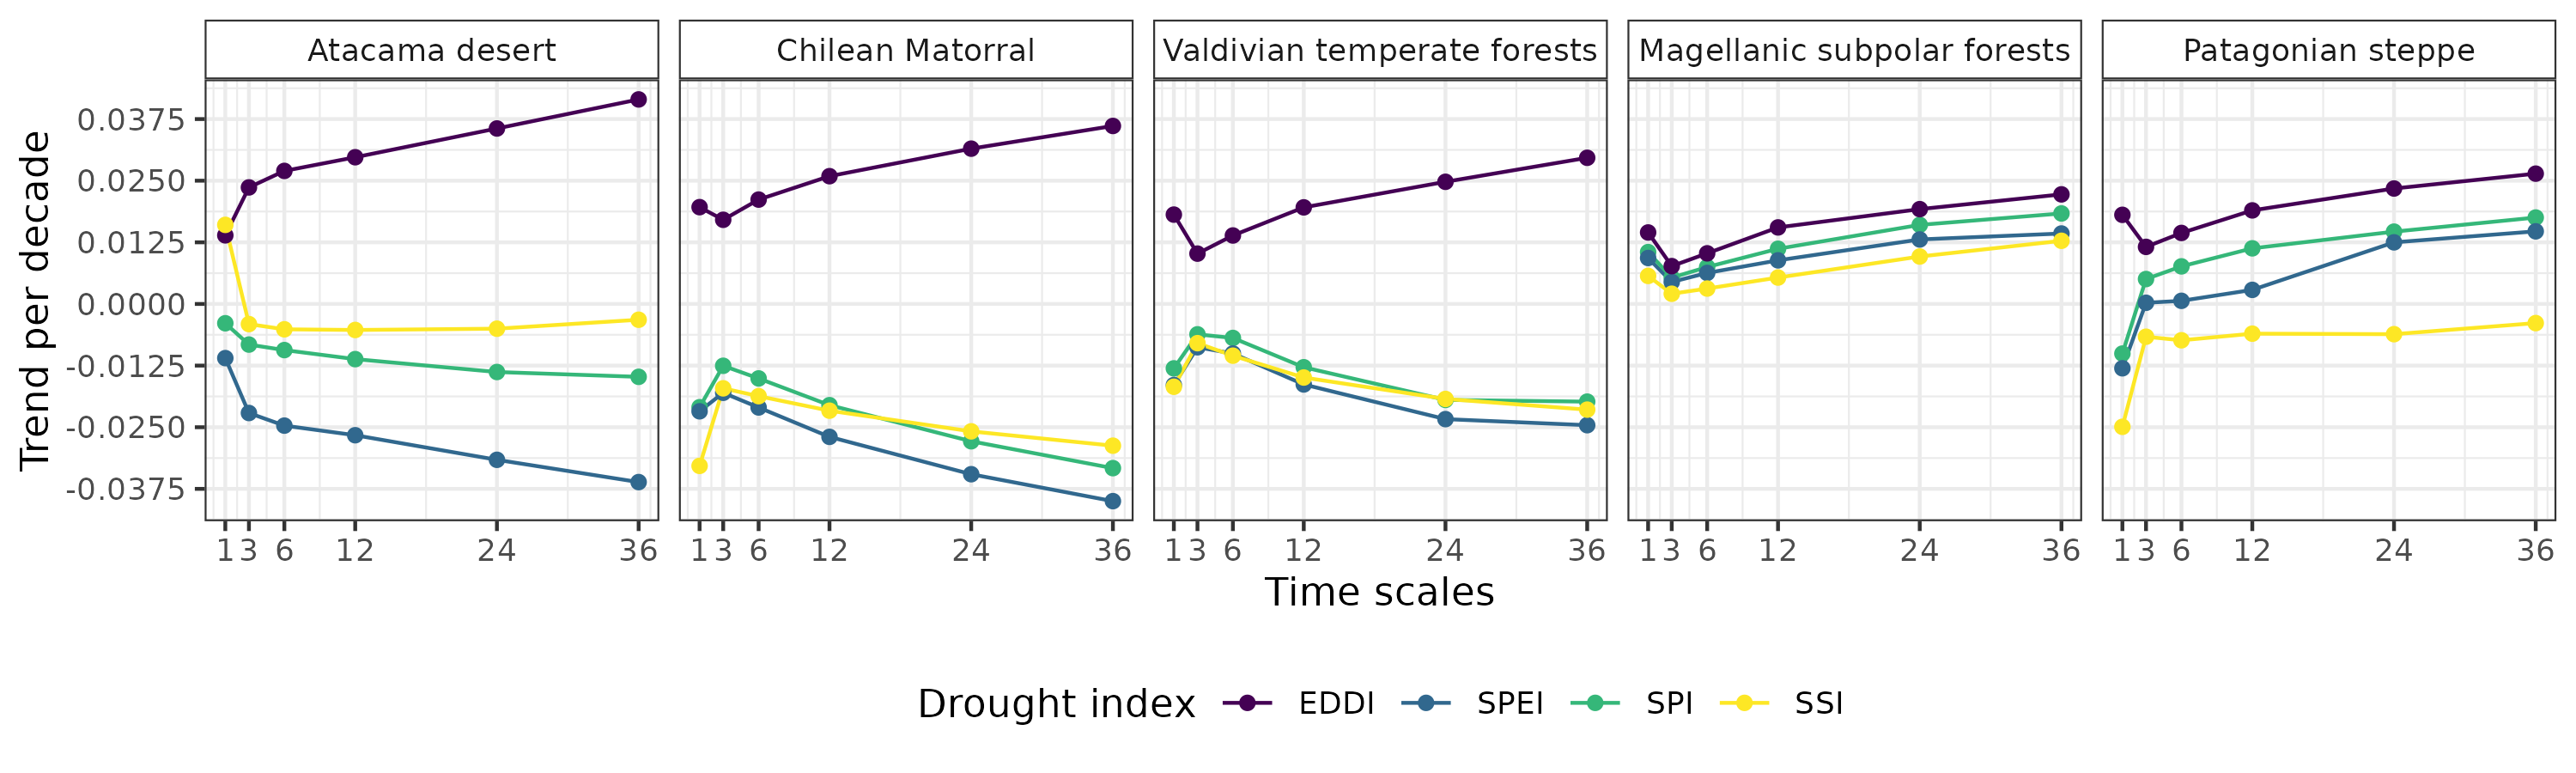
\includegraphics{../output/figs/trend_macrozone_drought_indices.png}

}

\caption{\label{fig-trendDIMacro}Trend per decade for the drought
indices SPI, EDDI, SPEI, and SSI aggregated by macrozone.}

\end{figure}

\blandscape

\begin{figure}

\begin{minipage}[t]{0.50\linewidth}

{\centering 

\raisebox{-\height}{

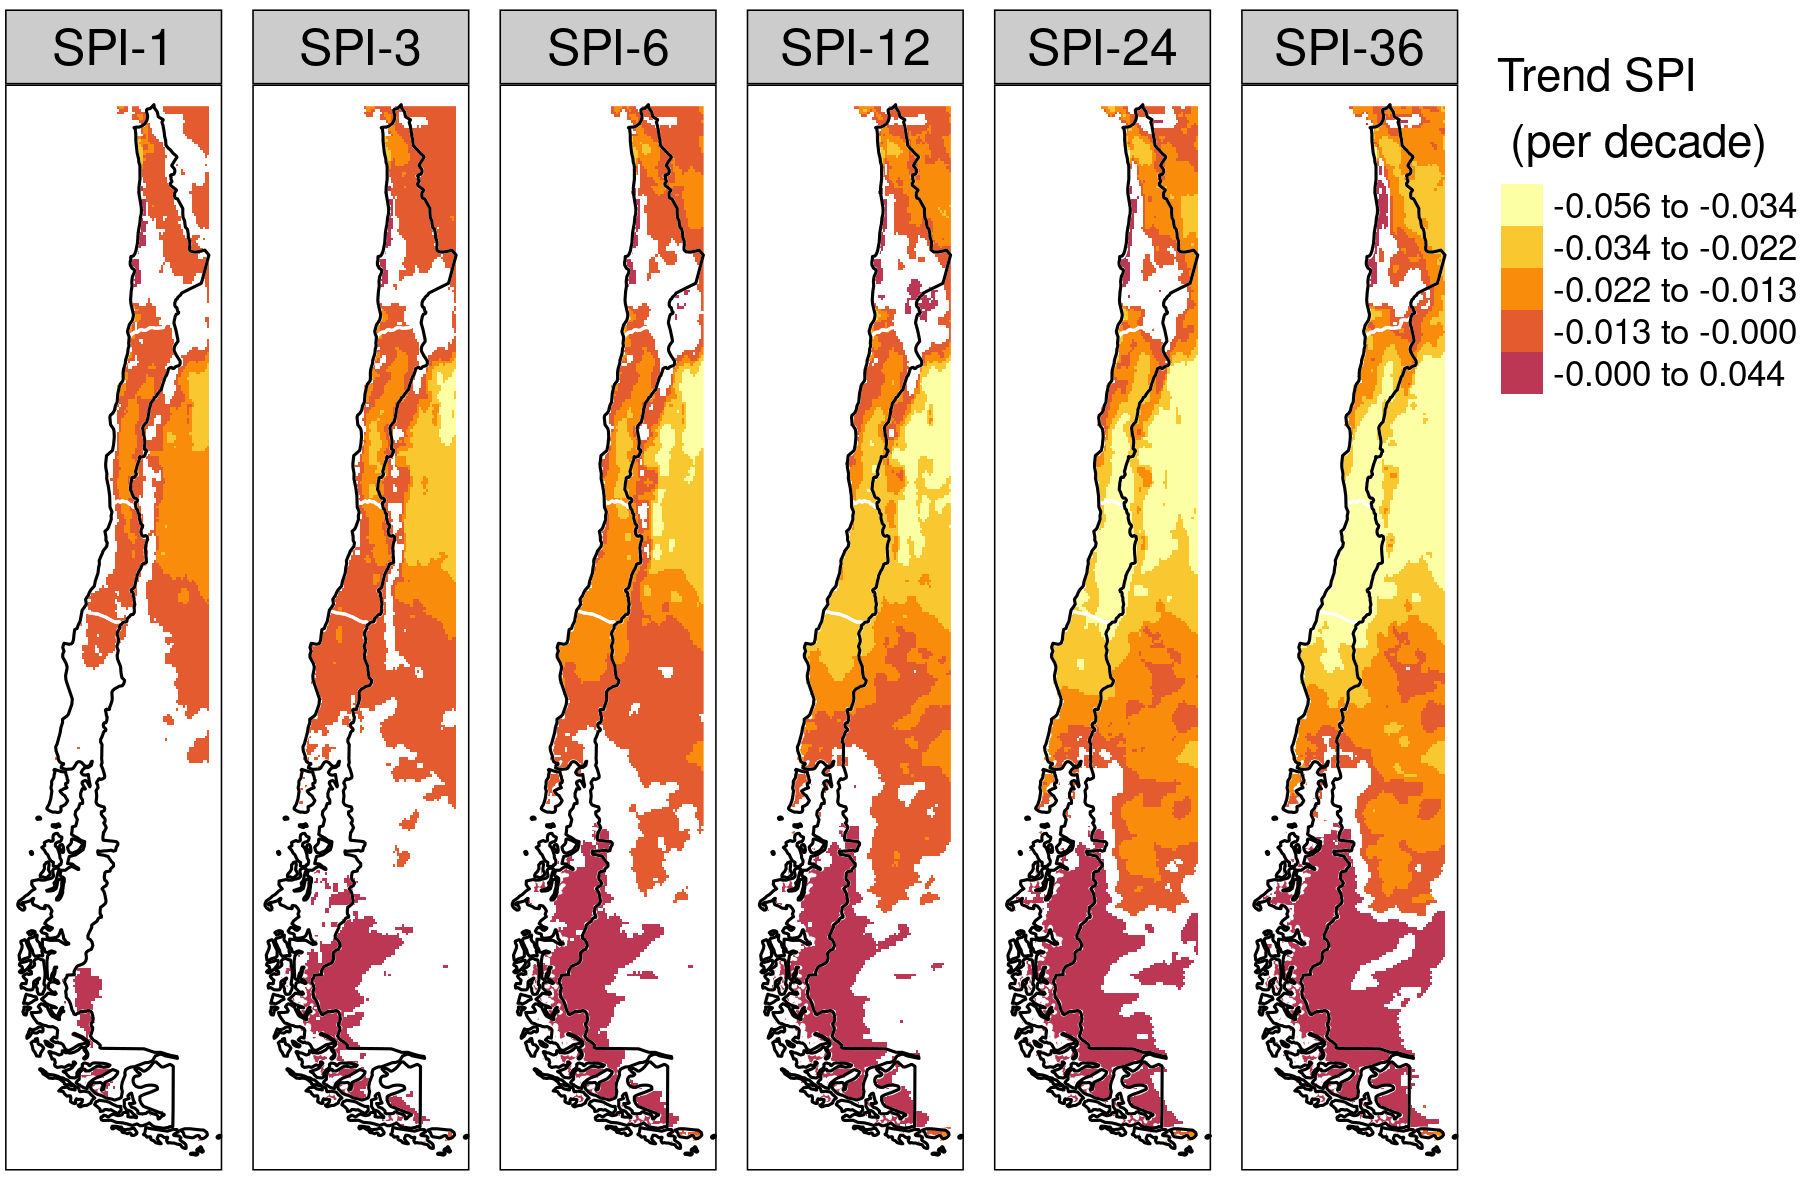
\includegraphics{../output/figs/trend_raster_SPI_1981-2023.png}

}

}

\subcaption{\label{fig-trendDI-1}SPI (Standardized Precipitation Index)}
\end{minipage}%
%
\begin{minipage}[t]{0.50\linewidth}

{\centering 

\raisebox{-\height}{

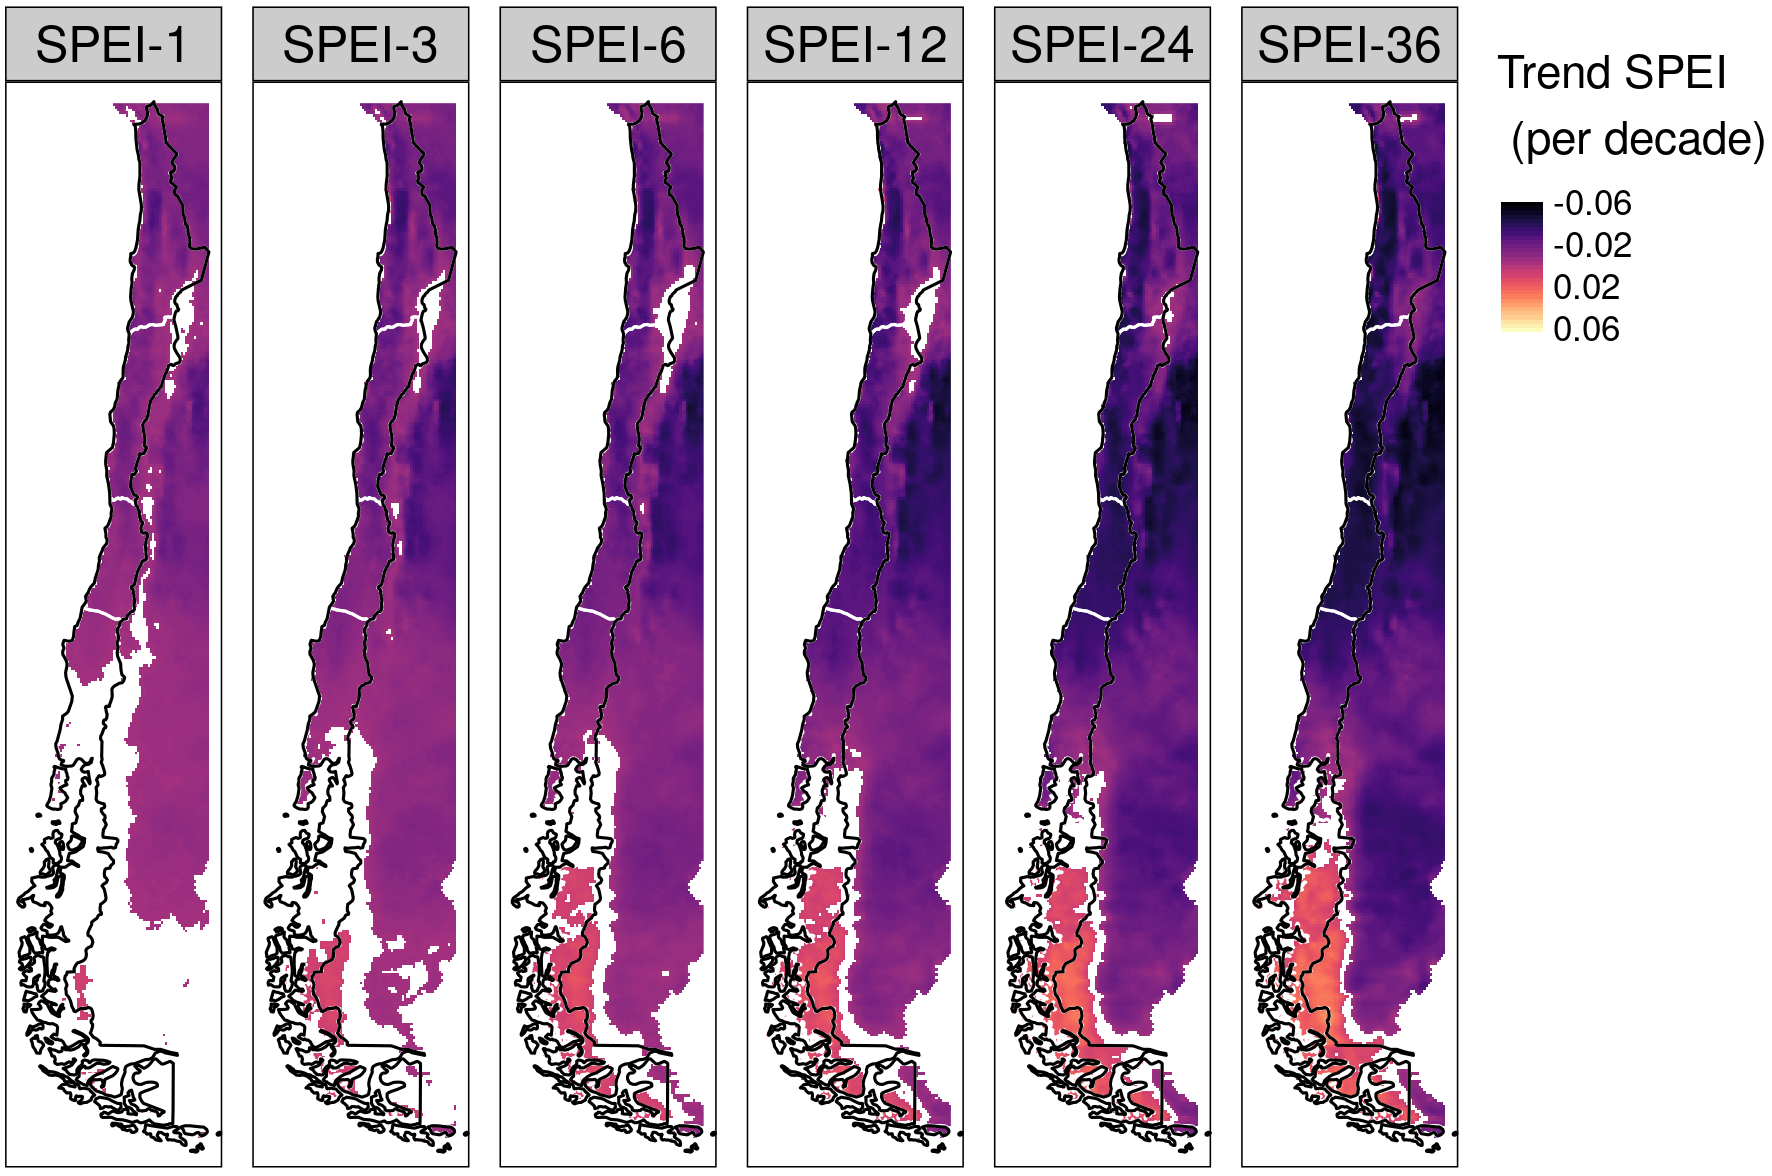
\includegraphics{../output/figs/trend_raster_SPEI_1981-2023.png}

}

}

\subcaption{\label{fig-trendDI-2}SPEI (Standardized Precipitation
Evapotranspiration Index)}
\end{minipage}%
\newline
\begin{minipage}[t]{0.50\linewidth}

{\centering 

\raisebox{-\height}{

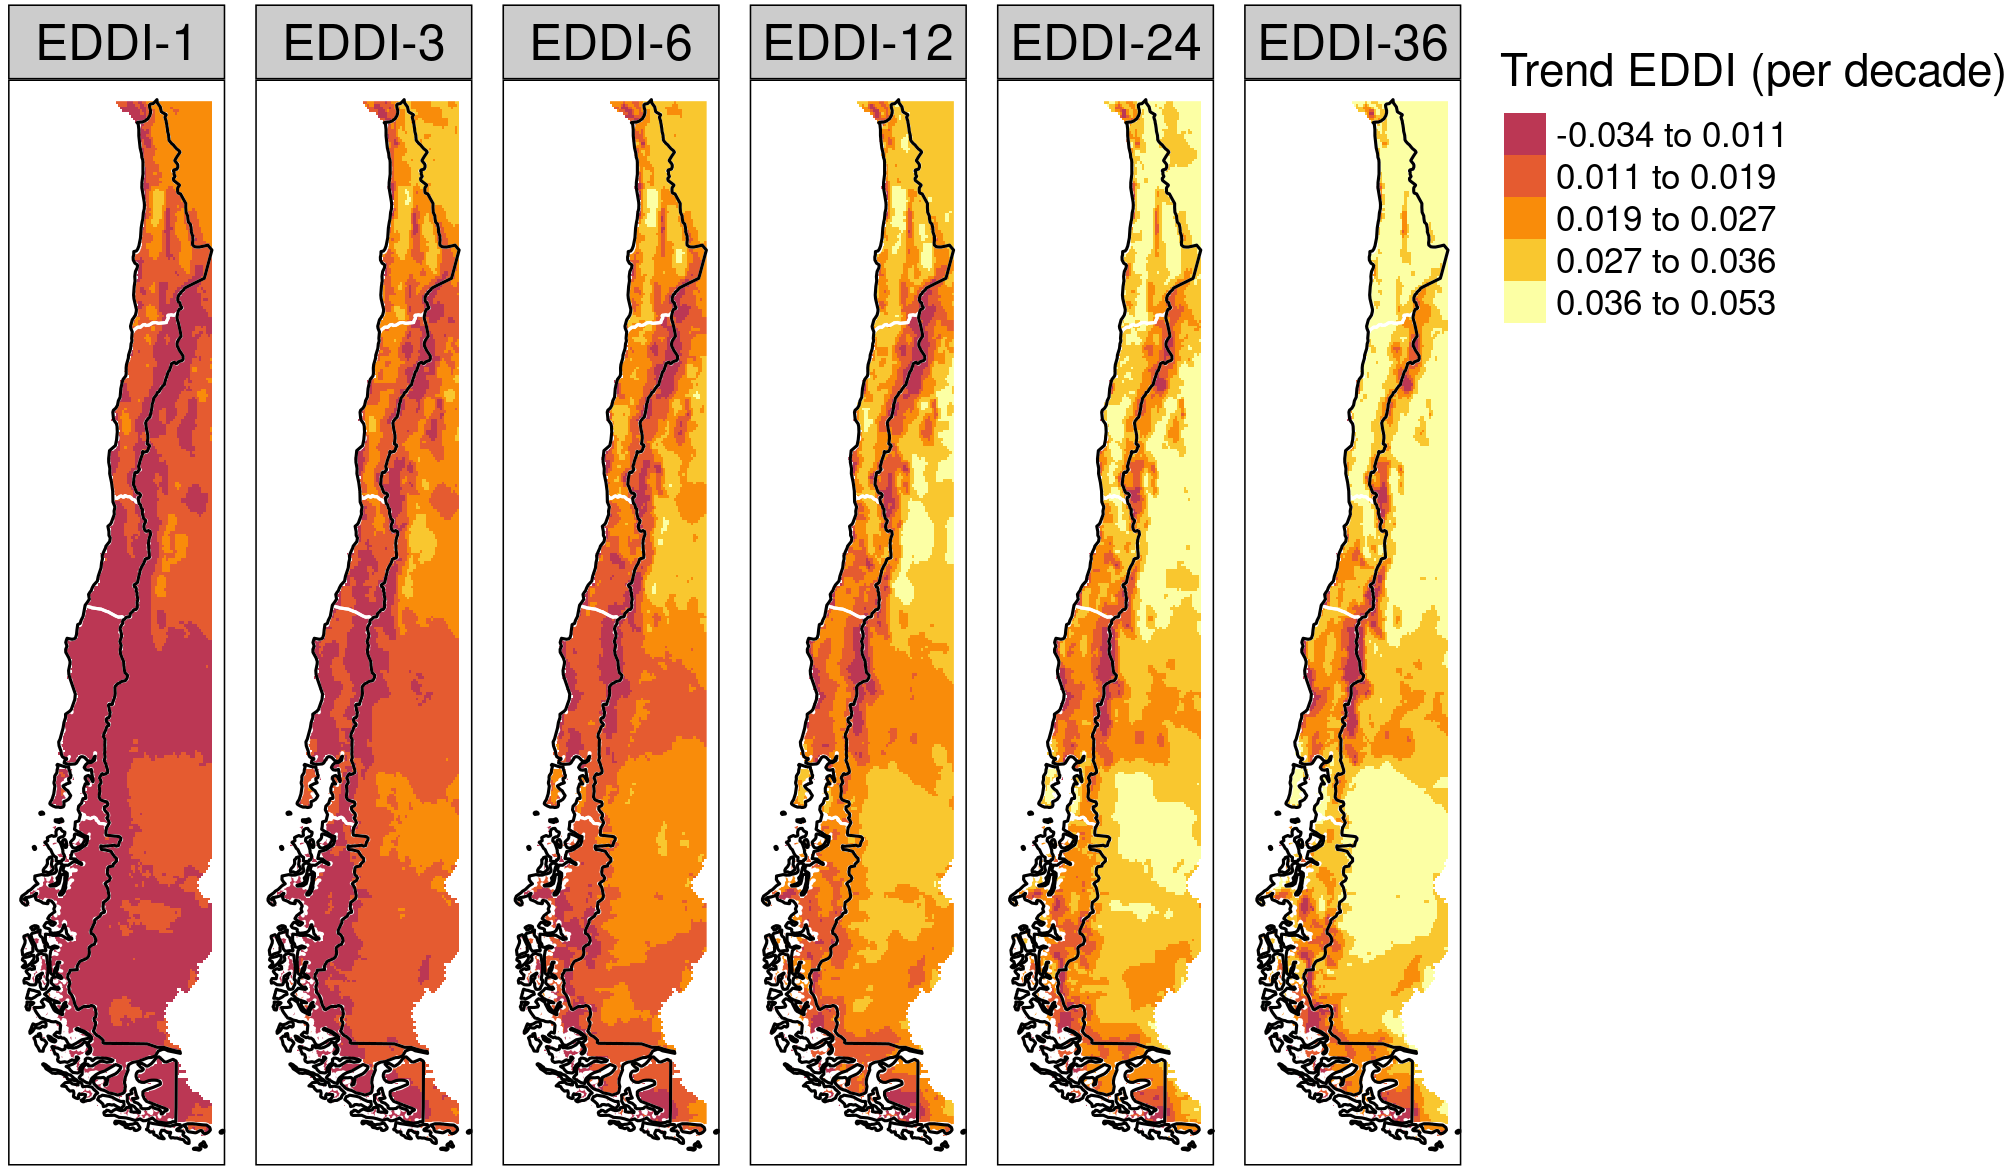
\includegraphics{../output/figs/trend_raster_EDDI_1981-2023.png}

}

}

\subcaption{\label{fig-trendDI-3}EDDI (Evaporative Demand Drought
Index)}
\end{minipage}%
%
\begin{minipage}[t]{0.50\linewidth}

{\centering 

\raisebox{-\height}{

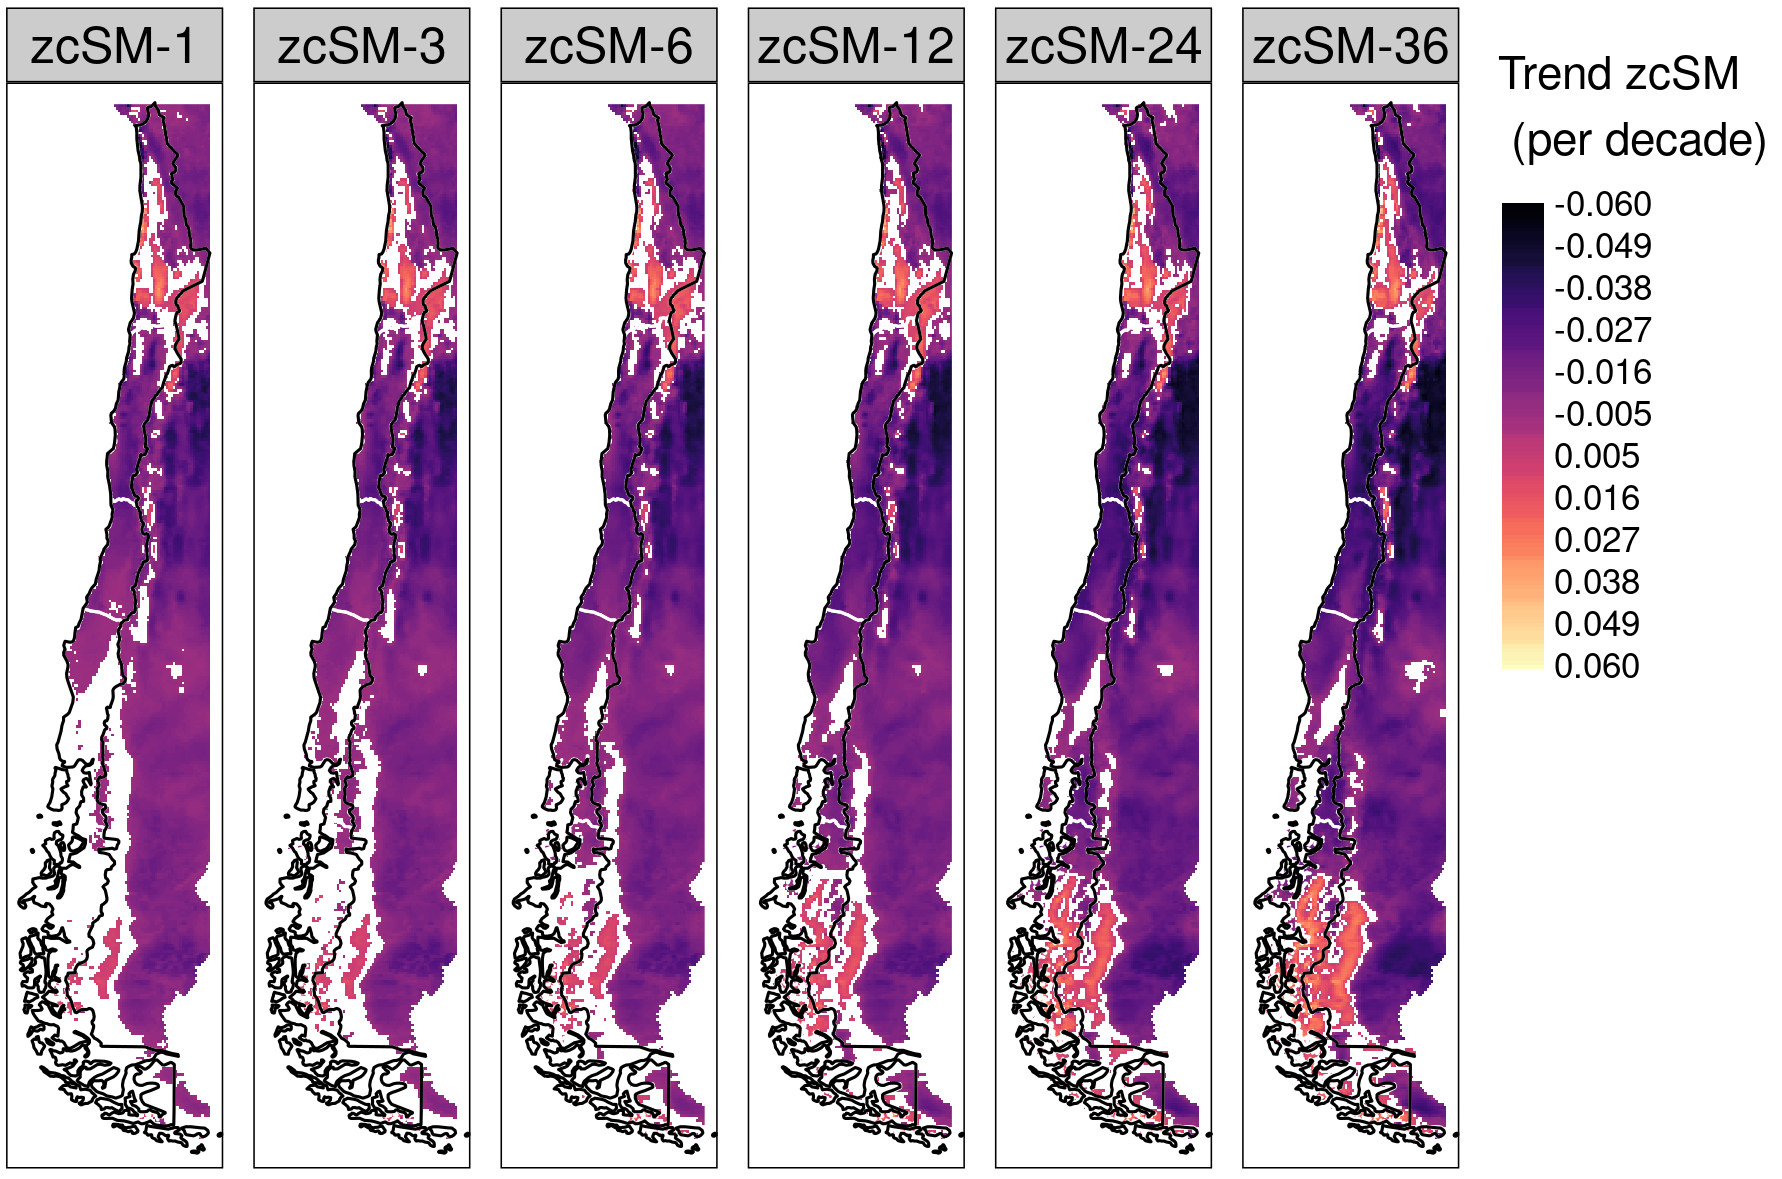
\includegraphics{../output/figs/trend_raster_zcSM_1981-2023.png}

}

}

\subcaption{\label{fig-trendDI-4}SSMI (Standardized Soil Moisture
Index)}
\end{minipage}%

\caption{\label{fig-trendDI}Linear trend of the drought index (*) at
time scales of 1, 3, 6, 12, 24, and 36 months for 1981-2023}

\end{figure}

\elandscape

\begin{table}[!ht]
\caption{Summarry per land cover macroclass and macrozone regarding the correlation between zcNDVI with the drought indices EDDI, SPI, SPEI, and SSI for time scales of 1, 3, 6, 12, 24, and 36. The numbers in each cell indicate the time scale that reached the maximum correlation for the land cover and macrozone, and the color indicates the strength of the r-squared obtained with the index and the time scale.}
\label{tab-corlandcover}
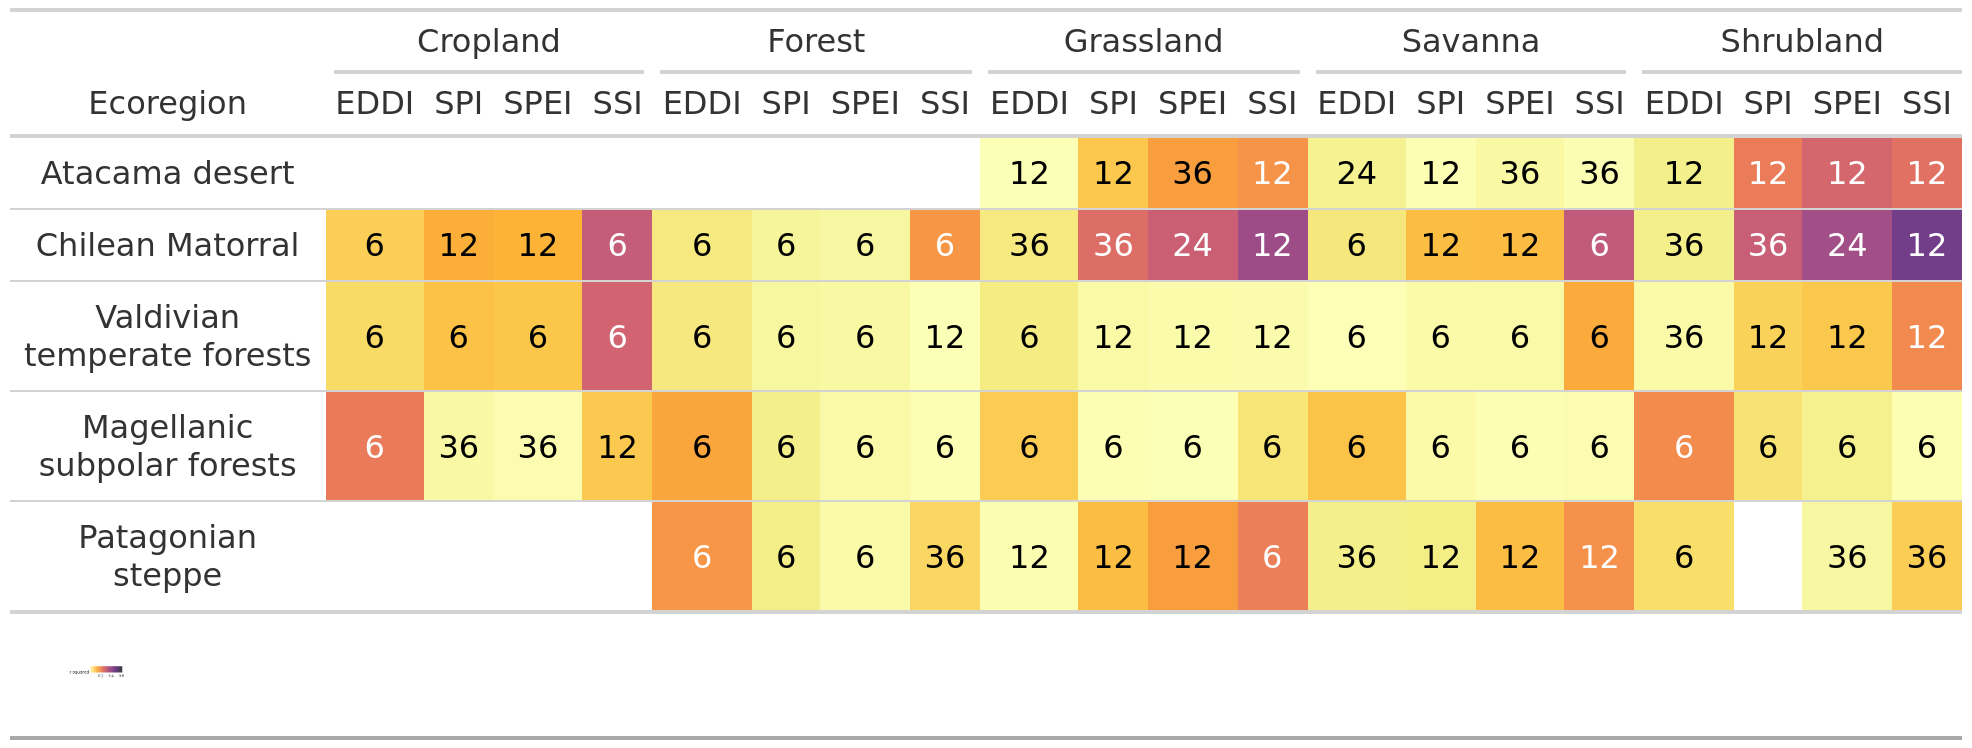
\includegraphics[]{../output/figs/tabla_r_cor_macro_indice.png}
\end{table}

Analyzing the water supply, the macrozones that have the lowest trend
are ``Norte Chico'' and ``Centro,'' where the SPI, SPEI, and SSI show
that it decreases at longer time scales due to the prolonged reduction
in precipitation. At 36 months, it reaches trends between -0.03 and
-0.04 (z-score) per decade for SPI, SPEI, and SSI
(Figure~\ref{fig-trendDI}). For ``Sur,'' the behavior is similar,
decreasing at longer scales and having between -0.016 and -0.025 per
decade for SPI, SPEI, and SSI. On the other hand, all macrozones show an
increase in the trend in all the drought indices, with ``Norte Grande''
having the highest at 36 months (0.042 per decade). Because of this, the
SPEI (which uses AED) reached its lowest value in ``Norte Grande,'' with
-0.03 at 36 months. Despite the other macrozones, ``Austral'' showed an
increase in all indices, being the highest for EDDI at 36 months (0.025)
and the lowest for SSI, which shows only a minor increase in the trend
(Figure~\ref{fig-trendDI} and Figure~\ref{fig-trendDIMacro}).

\hypertarget{impact-for-water-supply-and-demand-and-soil-moisture-in-vegetation-productivity}{%
\subsection{Impact for water supply and demand, and soil moisture in
vegetation
productivity}\label{impact-for-water-supply-and-demand-and-soil-moisture-in-vegetation-productivity}}

According to what is shown in Figure~\ref{fig-corTimeScale},
Figure~\ref{fig-corPerson}, and Table \ref{tab-corlandcover}, forest
seems to be the most resistant type to drought. Showing that only
``Centro'' is slightly (rsq = 0.25) impacted by a 12-month soil moisture
deficit (SSI-12). In the ``Norte Chico'' and to a lesser extent in the
``Norte Grande,'' it is evident that a SSI-12 with a rsq = 0.45 and a
decrease in water supply (SPI-36 and SPEI-24 with rsq = 0.28 and 0.34,
respectively) have an impact on grasslands. However, this type was
unaffected by soil moisture, water supply, or demand in macrozones
further south. The types that show to be most affected by variation in
climate conditions are shrublands, savannas, and croplands. For savannas
in ``Norte Chico,'' the SSI-12 and SPI-24 reached an rsq of 0.74 and
0.58, respectively. This value decreases to the south, but the SSI-12 is
still the variable explaining more of the variation in vegetation
productivity (rsq = 0.45 in ``Centro'' and 0.2 in ``Sur''). In the case
of croplands, the SPEI-12, SPI-36, and SSI-12 explain between 45\% and
66\% of ``Norte Chico.'' The type of land most impacted by climatic
variation was shrubland, where soil moisture explained 59\% and
precipitation, 37\%, in ``Norte Chico'' and ``Centro,'' with SSI-12
being the most relevant variable, then SPI-36 in ``Norte Chico'' and
SPI-24 in ``Sur.''

\begin{figure}[!ht]

{\centering 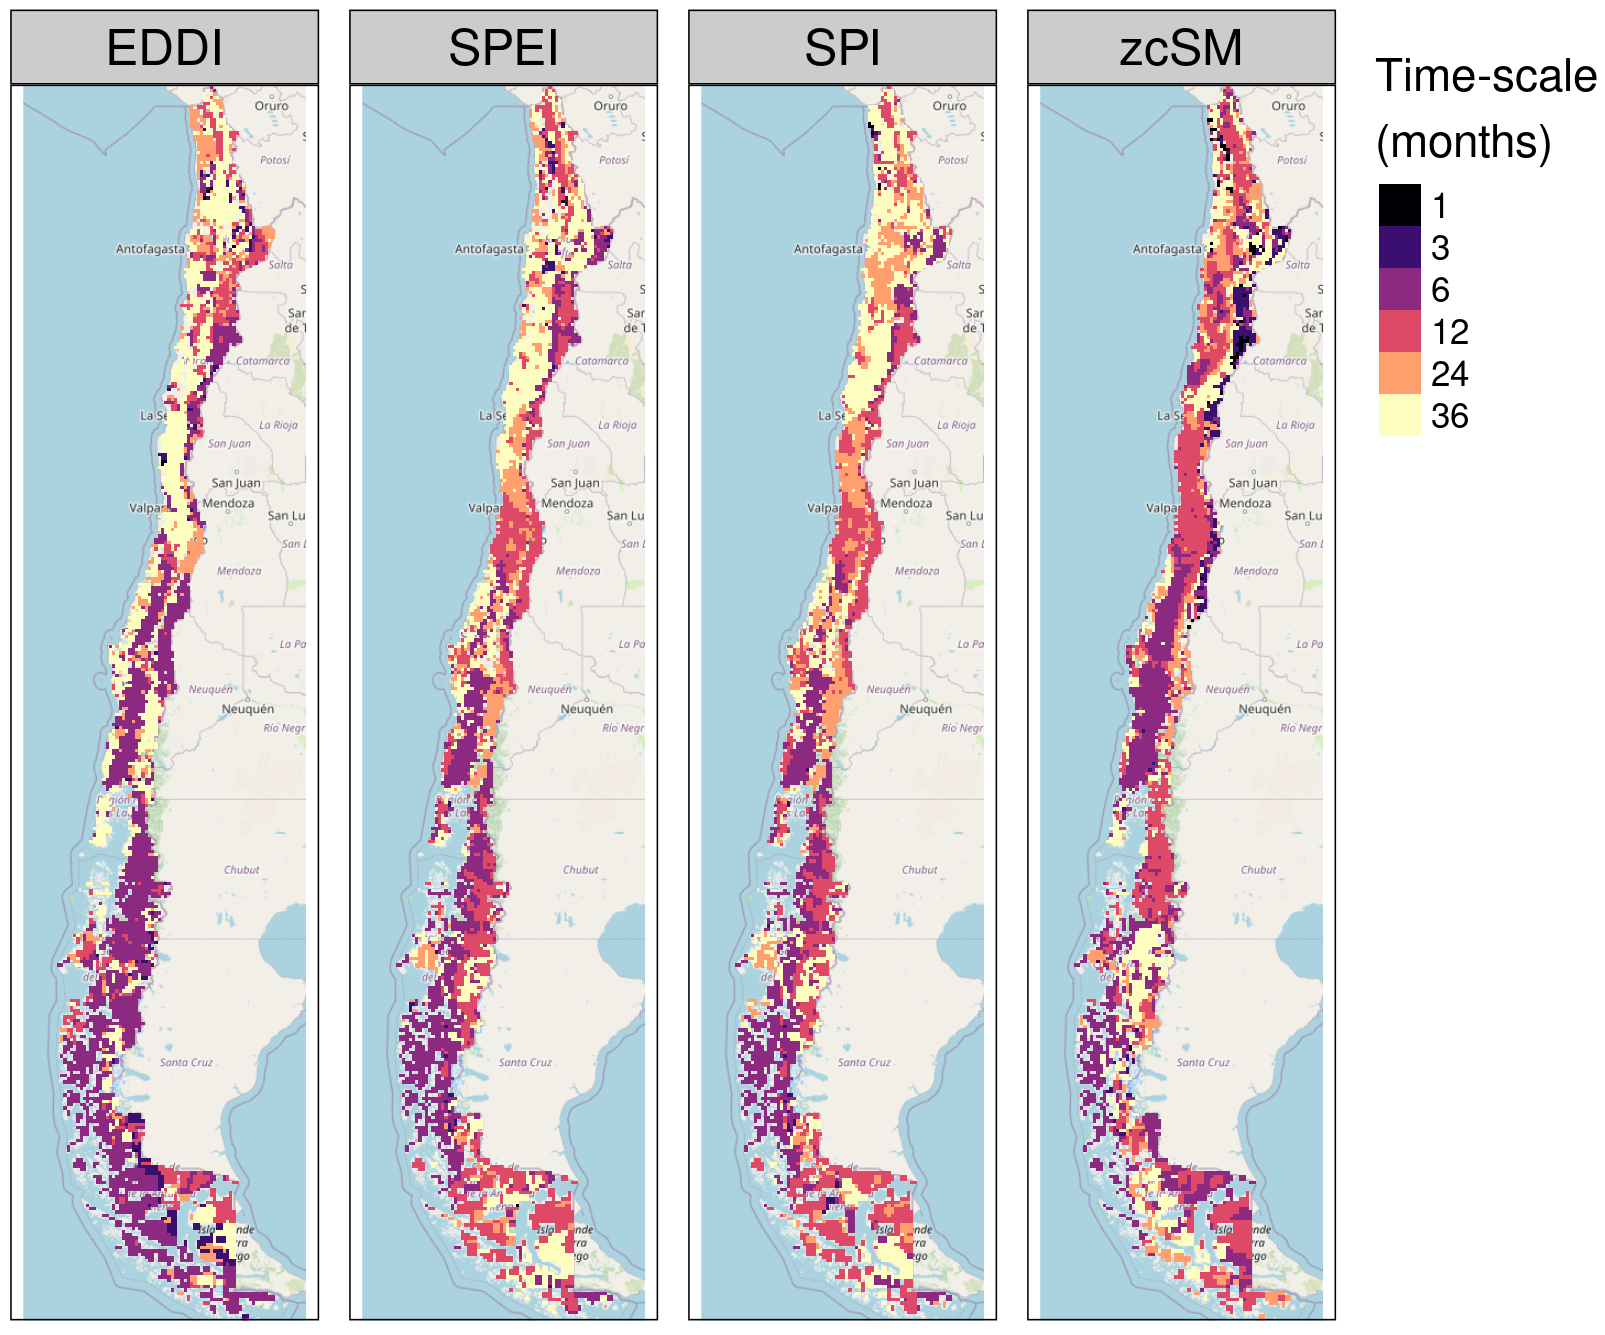
\includegraphics{../output/figs/mapa_cor_selec_indices_zcNDVI6.png}

}

\caption{\label{fig-corTimeScale}Time scales per drought index that
reach the maximum coefficient of determination}

\end{figure}

\begin{figure}[!ht]

{\centering 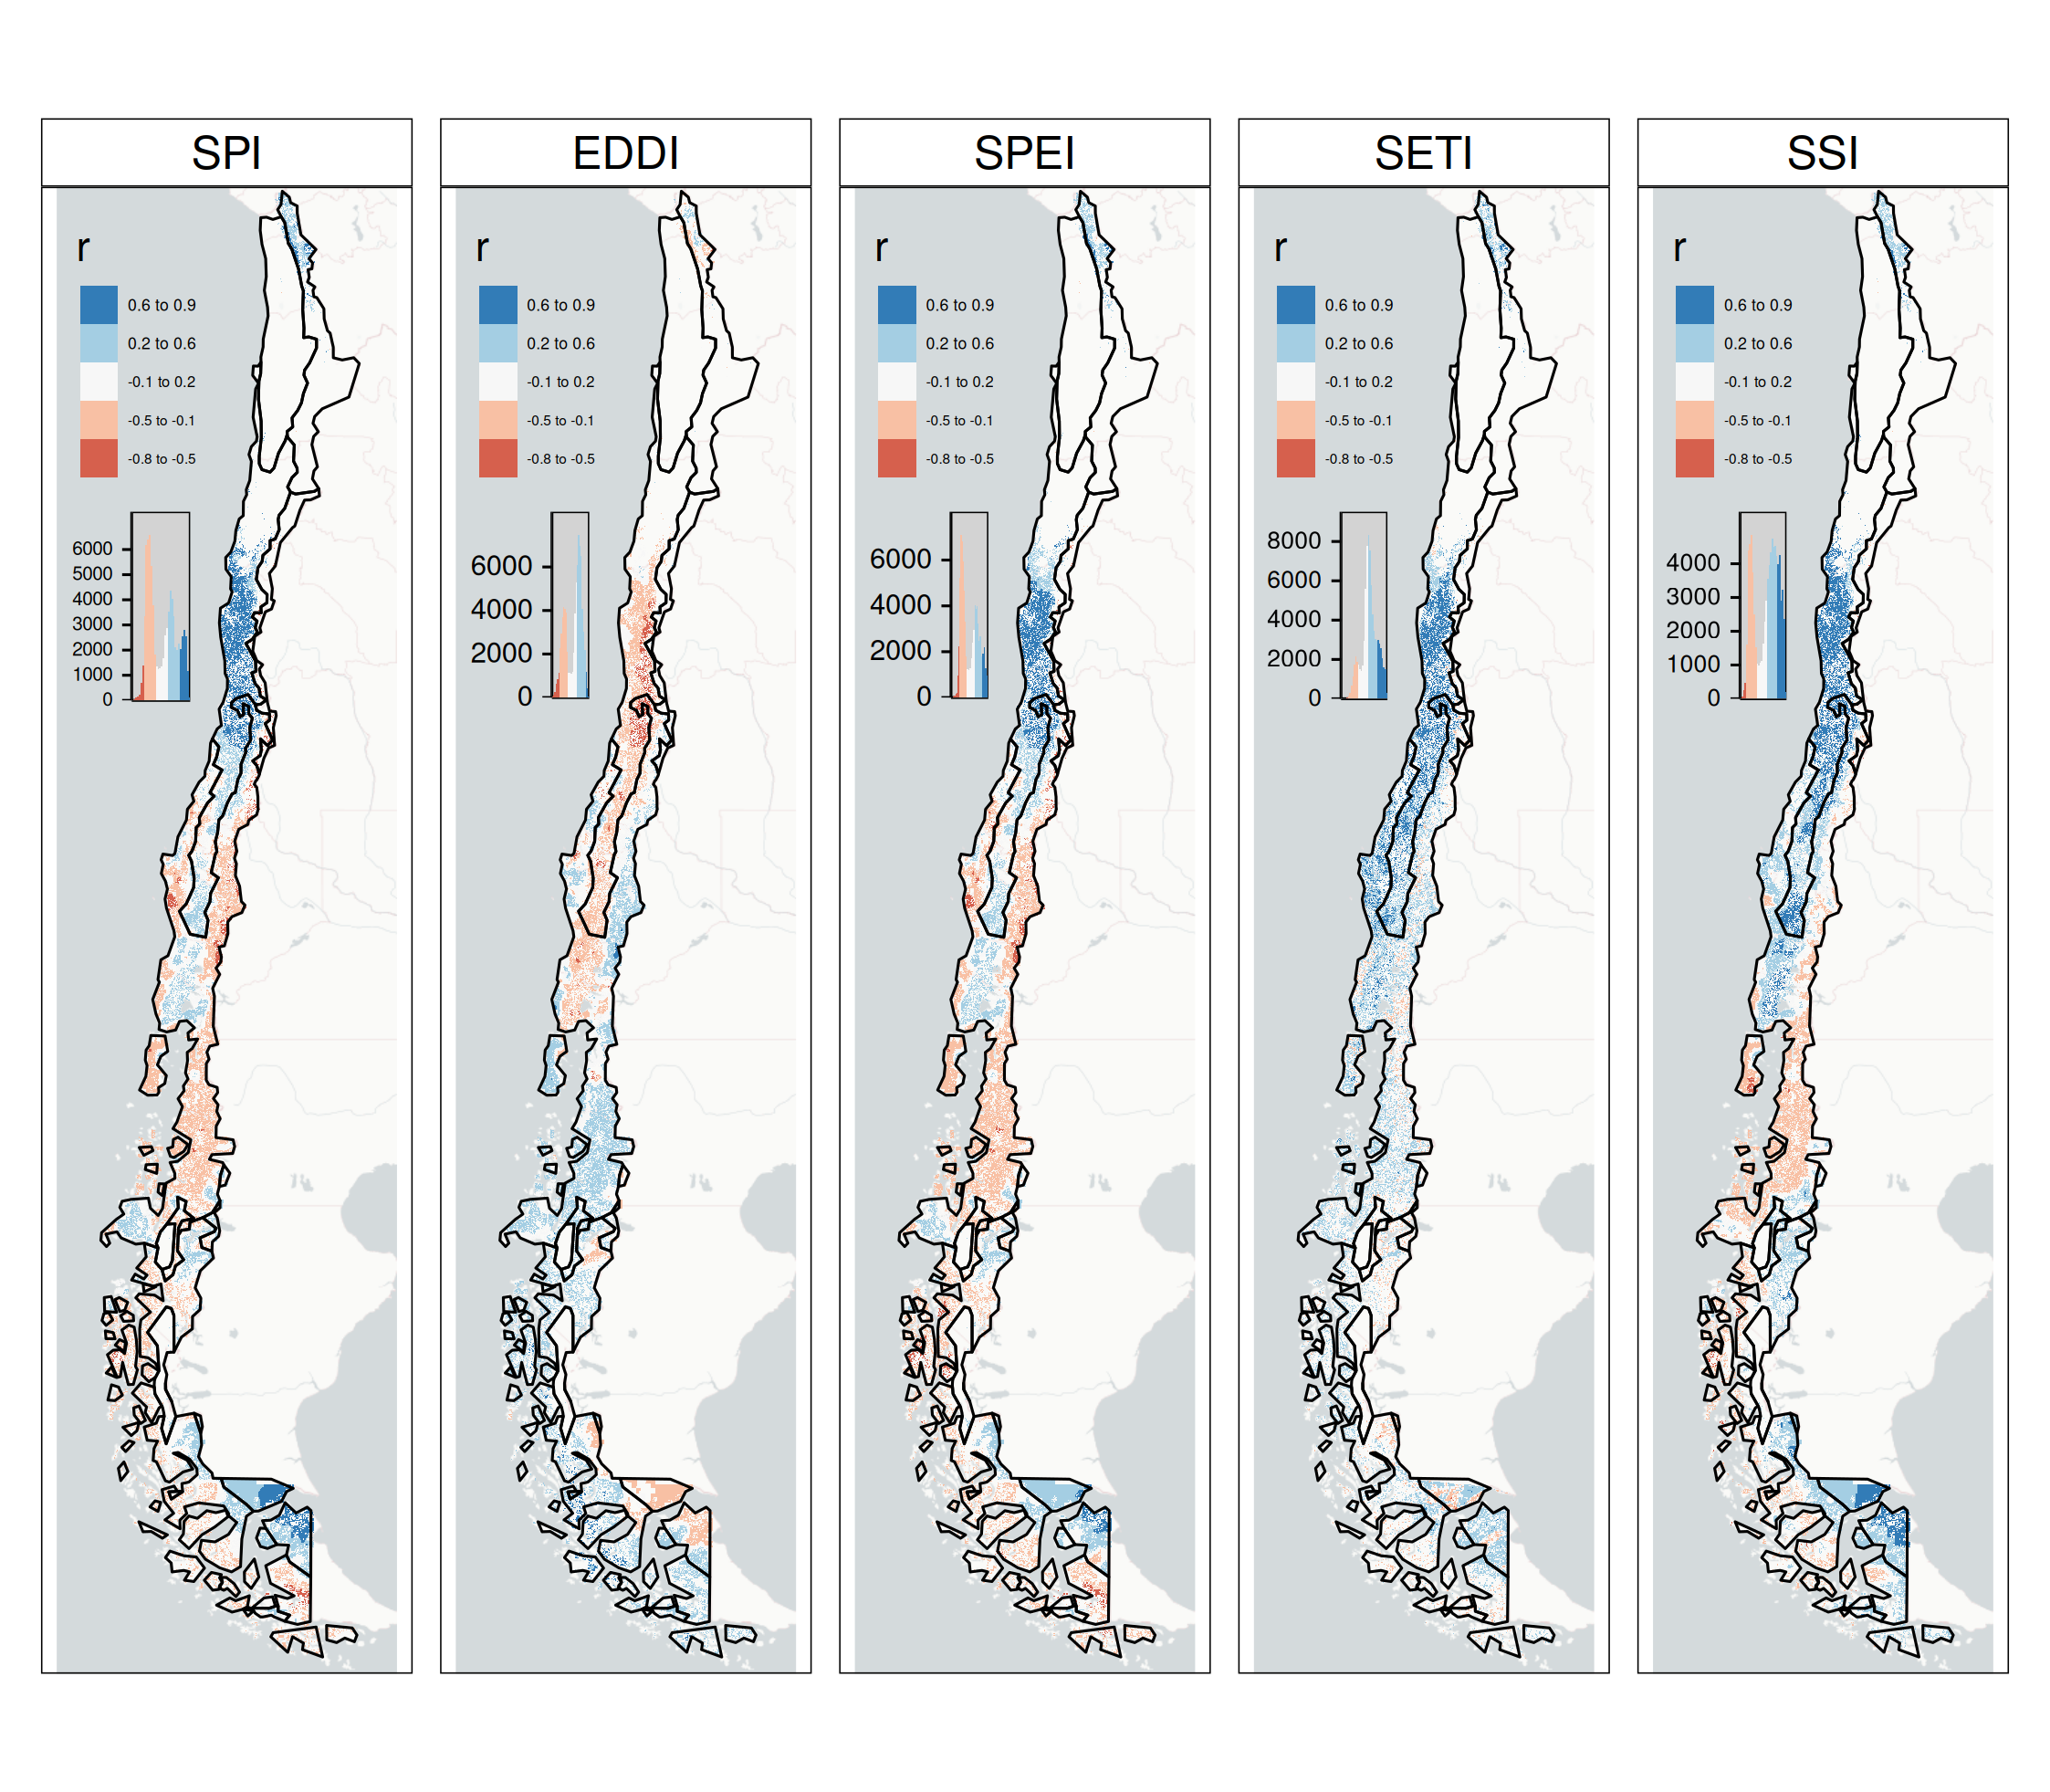
\includegraphics{../output/figs/mapa_cor_r_indices_zcNDVI6.png}

}

\caption{\label{fig-corPerson}Pearson correlation value for the time
scales and drought index that reach the maximum coefficient of
determination}

\end{figure}

\hypertarget{discussion}{%
\section{Discussion}\label{discussion}}

\hypertarget{drought-trend-and-attribution-to-lulcc}{%
\subsection{Drought trend and attribution to
LULCC}\label{drought-trend-and-attribution-to-lulcc}}

\citet{Vicente-Serrano2021}, in a study at the global scale of drought
trends, indicates that there have not been significant trends in
meteorological drought since 1950. Also, state that the increase in
hidrological trend in some parts of the globe (northeast Brazil and the
Mediterranean region) is related to changes in land cover and
specifically to the rapidly increasing irrigated area, which
consequently increases water extraction. \citet{Kogan2020} analyzed the
agricultural drought impact globally and in the main grain producer
countries, finding that \emph{``since 1980, the Earth warming has not
changed the drought area or intensity''}.

In our study, we considered the variation in vegetation productivity in
Chile for areas without changes in land cover macroclasses (see
Section~\ref{sec-persistence_mask}), to avoid misleading conclusions
that could be related to the increase in water demand due to LULCC. Our
results show a contrasting perspective. There has been a significant
trend in the decline of vegetation productivity (zcNDVI) since 2000 for
``Norte Chico'' and ``Centro,'' which has been extreme between 2020 and
2022, seemsly due to an intense hydrological drought due to the
persistance of the Mega Drought \citep{Garreaud2017}. Despite using the
persistance mask for vegetation's trend analysis, cropland, which is the
most water-demand type, showed a decrease trend in ``Norte Chico'' and
``Centro.'' Also, there was an increase in barren land for both types.
These changes are associated with a decrease in water demand from
vegetation. Nonetheless, we used the persistant land cover to ensure
that the pixel has the same class; in the case of croplands, it could
happen that some areas had changed crops for others with higher water
consumption. But this effect should be minor compared to the results
from ladcover macroclasses.

On the other hand, for ``Norte Chico'' and ``Centro,'' our results show
a decrease in trends of water supply (SPI and SSI), which are higher at
larger time scales and consequently impact the hydrological system. We
claim that what occurred in central Chile defies findings made at the
global level \citep{Vicente-Serrano2021, Kogan2020}, demonstrating that
a constant decrease in water supply rather than an increase in water
demand (i.e., irrigated crops) is the main cause of the hydrological
drought. Finally, central Chile has shown a diminishment in vegetation
productivity for all macroclasses, mainly attributed to variation in
water supply, i.e., precipitation, which could be strengthened by an
increase in water demand by, for example, an increase in the surface
area of irrigated crops.

\hypertarget{land-cover-types-and-their-impact-by-drought}{%
\subsection{Land cover types and their impact by
drought}\label{land-cover-types-and-their-impact-by-drought}}

We found that shrubland, savannas (Chilean matorral), and croplands are
the most sensitive to climate conditions. Being most affected by the
12-month soil moisture deficit. In a study in the Yangtze River Basin in
China, Jiang2020 analyzed the impact of drought on vegetation using the
SPEI and the Enahanced Vegetation Index (EVI). They found that cropland
was more sensitive to drought than cropland, showing that cropland
responds strongly to short- and medium-term drought (\textless{}
SPEI-6). In our case, the SPEI-12 was the one that most impacted the
croplands in ``Norte Chico'' and ``Centro.'' In general, most studies
show that croplands are most sensitive to short-term drought
(\textless{} SPI-6)
\citep{Zambrano2016, Potopova2015, Dai2020, Rhee2010}. Short-term
precipitation deficits impact soil water, and thus less water is
available for plant growth. However, we found that in ``Norte Chico,''
an SPI-36 and SPEI-12 had a higher impact, which are associated with
hydrological drought (long-term), and in ``Centro,'' an SPI-12 and
SPEI-12. Thus, we attribute this impact to the hydrological drought that
has decreased groundwater storage \citep{Taucare2024}, which in turn is
impacted by long-term deficits, and consequently, the vegetation is more
dependent on groundwater. In ``Sur'' and ``Austral,'' the correlations
between drought indices and vegetation productivity decrease, as do the
time scales that reach the maximum r-squared (\ref{tab-corlandcover}).
What can be explained is that, south of ``Centro,'' predominate forest
and grassland, the most resistant types. Also, drought episodes have
been less frequent and intense. The drought episodes have had a lower
impact on water availability for vegetation.

Extreme drought conditions are an important driver of tree mortality, as
shown by \citet{Senf2020} in Europe. However, we found that forest is
the type of land cover macroclass less affected by variation in drought
indices, being the most resistant land cover class to drought.
Supporting this is \citet{Fathi-Taperasht2022}, who asserts that Indian
forests are the most drought-resistant and recover rapidly. Similarly,
the work of \citet{Wu2024}, who analyzed vegetation loss and recovery in
response to meteorological drought in the humid subtropical Pearl River
basin in China, indicates that forests showed higher drought resistance.
Using Vegetation Optical Depth (VOD), kNDVI, and EVI, \citet{Xiao2023},
tests the resistance of ecosystems and finds that ecosystems with more
forests are better able to handle severe droughts than croplands. They
attribute the difference to a deeper rooting depth of trees, a higher
water storage capacity, and different water use strategies between
forest and cropland \citep{Xiao2023}.

In contrast to what we obtained, \citet{Venegas2022}, who studied
Cryptocarya alba and Beilschmiedia miersii (both from the Lauraceae
family) that live in sclerophyllous forests in Chile, found that the
trees' overall growth had slowed down. This could mean that the natural
dynamics of their forests have changed. They attributed it to the
cumulative effects of the unprecedented drought (i.e., hydrological
drought). Thus, we attribute that forest to being the most resistant to
drought, due to the fact that most of the species comprising it are
highly resilient to water scarcity compared to the other land cover
classes. Nonetheless, if we want to go deep in our analysis, we should
use earth observation data that is able to capture a higher level of
detail. For example, when we used MOD13A3 with a 1km spatial resolution
to measure vegetation condition, it took the average condition of 1
square kilometer. Then, to study how a type of forest (e.g.,
sclerophyllous forest) changes in response to drought on a local level
using remote sensing, we should use operational products with higher
spatial resolutions, such as those from Landsat or Sentinel.

\hypertarget{soil-moisture-vegetation-productivity-and-agricultural-drought.}{%
\subsection{Soil moisture, vegetation productivity, and agricultural
drought.}\label{soil-moisture-vegetation-productivity-and-agricultural-drought.}}

The main external factors that affect biomass production by vegetation
are ET and SM, and the rate of ET in turn depends on the availability of
water storage in the root zone. Thus, soil moisture plays a key role in
land carbon uptake and, consequently, in the production of biomass
\citep{Humphrey2021}. Moreover, \citet{Zhang2022} indicates there is a
bidirectional causality between soil moisture and vegetation
productivity. Lastly, some studies have redefined agricultural drought
as soil moisture drought from an hydrological perspective
\citep{Loon2016, Samaniego2018}. Even though soil moisture is the
external factor most determinant of vegetation biomass, there are
multiple internal factors, such as species, physiological
characteristics, and plant hydraulics, that would affect vegetation
productivity. Because of that, we believe that agricultural drought,
referring to the drought that impacts vegetation productivity, is the
most proper term, as originally defined by \citet{Wilhite1985}.

The study results showed that the soil moisture-based drought index
(SSI) was better at explaining vegetation productivity across land cover
macroclasses than meteorological drought indices like SPI, SPEI, and
EDDI. In the early growing season and especially in irrigated rather
than rainfed croplands, soil moisture has better skills than SPI and
SPEI for estimating gross primary production (GPP), according to
\citet{Chatterjee2022}'s evaluation of the SPI and SPEI and their
correlation with GPP in the CONUS. Also, \citet{Zhou2021} indicates that
the monthly scaled Standardized Water Deficit Index (SWDI) can
accurately show the effects of agricultural drought in most of China.
Complementary, \citet{Nicolai2017} analyzed the time-lag between SWDI
and the Vegetation Condition Index (VCI), and they state that there was
no or little time-lag with croplands but a significant time-lag in the
case of forests.

In our case, there is strong spatial variability throughout Chile and
between classes, mainly attributable to climate heterogeneity,
hydrological status, or vegetation resistance to water scarcity. The
semi-arid ``Norte Chico'' and the Mediterranean ``Centro'' were where
SSI had the best performance. In Chile, medium-term deficits of 12
months are more relevant in the response of vegetation, which decreases
to the south, and in the case of croplands, they seem to react in a
shorter time, with six months (SSI-6) in ``Centro.'' This variation for
croplands could be related to the fact that in ``Norte Chico,'' the
majority of crops are irrigated, but to the south there is a higher
proportion of rainfed agriculture, which is most dependent on the
short-term availability of water. Rather, in the ``Norte Chico,'' the
orchards are more dependent on the storage of water in dams of
groundwater reservoirs, which are affected by long-term drought (e.g.,
SPI-36).

\hypertarget{early-drought-forecasting-for-vegetation-productivity}{%
\subsection{Early drought forecasting for vegetation
productivity}\label{early-drought-forecasting-for-vegetation-productivity}}

We analyzed the correlation between meteorological and soil moisture
drought indices with zcNDVI. From our findings, we could further use the
drought indices and time scales that have the highest r-squared to
develop a combined model to forecast vegetation productivity in Chile.
Despite the fact that SSI was the best-performing index, the rest of the
indices should help to enhance predictability. \citet{Zambrano2018}
proposed a prediction model for cropland surface in Chile at
administrative units with a 1- to 6-month lead time using zcNDVI from
MODIS and climate oscilation indices. The results given were r-squared,
ranging from 0.95 at a 1-month lead time to 0.37 at a 6-month lead time.
Thus, incorporating the results of this study with those made by
\citet{Zambrano2018}, we could develop a combined forecasting model at
the pixel level for the macroclasses in Chile based on drought indices
of water demand and supply and soil moisture.

\hypertarget{future-outlook-to-complete}{%
\subsection{Future outlook (to
complete)}\label{future-outlook-to-complete}}

\hypertarget{conclusion}{%
\section{Conclusion}\label{conclusion}}

There is a trend toward decreasing water supply in most parts of Chile,
less in the ``Austral,'' which is stronger in the ``Centro'' and ``Norte
Chico.'' The whole country showed an increase in water demand.
Vegetation productivity only showed a decrease in the ``Norte Chico''
and ``Centro,'' being highest for shrubland and croplands. Forest is the
land cover most resistant to drought, and shrubland and cropland are the
most sensitive.

A soil moisture deficit of 12 months (SSI-12) is highly correlated with
vegetation productivity for the land cover classes of shrubland,
savannas, croplands, and forest in ``Norte Chico'' and ``Centro.'' For
the southern part of the country with humid conditions, the correlation
with SSI decreases. Soil moisture overcomes the capacity to explain
vegetation productivity over the supply and demand drought indices in
the entire territory.

The variation in vegetation productivity appears to be associated with
climate variation rather than anthropogenic factors (e.g., an increase
in water demand by irrigated crops). Even though switching to more
demanding crops on the land could increase the impact of drought on
vegetation, this would need to be more thoroughly investigated, for
instance at the watershed level.

The results of this study could help in the development of a robust
forecasting system for land cover classes in Chile., helping to improve
preparedness for climate change impacts on vegetation.

\hypertarget{supplementary-material}{%
\section*{Supplementary material}\label{supplementary-material}}
\addcontentsline{toc}{section}{Supplementary material}


\renewcommand\refname{References}
  \bibliography{references.bib}


\end{document}
